 %------------------------------------------------------------------------------
% Template file for the submission of papers to IUCr journals in LaTeX2e
% using the iucr document class
% Copyright 1999-2013 International Union of Crystallography
% Version 1.6 (28 March 2013)
%------------------------------------------------------------------------------

\documentclass{iucr}              % DO NOT DELETE % 
\usepackage{bm}
% \usepackage{graphicx}
% \usepackage{tabularx}
% \usepackage{subfigure}
% \usepackage{afterpage}
% \usepackage{sansmath}
\usepackage{mathtools}
% \usepackage{parskip}
\usepackage{tikz}
% \usepackage{tikzorbital}
% \usepackage{setspace}
% \usepackage{xcolor}
% \usepackage{amssymb}
% \usepackage{bm}
\usepackage{amsmath}
% \usepackage{fancyhdr}
% \usepackage{rotating}
% \usepackage{siunitx}
\usepackage[hyphens,spaces,obeyspaces]{url}
\usepackage{color}


\newcommand{\todo}[1]{{\color{red}[TODO: "#1'']}}
\newcommand{\inblue}[1]{{\color{blue}#1}}
\newcommand{\inred}[1]{{\color{red}#1}}
\newcommand{\ingreen}[1]{{\color{green}#1}}



     %-------------------------------------------------------------------------
     % Infobrmation about journal to which submitted
     %-------------------------------------------------------------------------
     \journalcode{S}              % Indicate the journal to which submitted
                                  %   A - Acta Crystallographica Section A
                                  %   B - Acta Crystallographica Section B
                                  %   C - Acta Crystallographica Section C
                                  %   D - Acta Crystallographica Section D
                                  %   E - Acta Crystallographica Section E
                                  %   F - Acta Crystallographica Section F
                                  %   J - Journal of Applied Crystallography
                                  %   M - IUCrJ
                                  %   S - Journal of Synchrotron Radiation

\begin{document} % DO NOT DELETE THIS LINE

     %-------------------------------------------------------------------------
     % The introductory (header) part of the paper
     %-------------------------------------------------------------------------

     % The title of the paper. Use \shorttitle to indicate an abbreviated title
     % for use in running heads (you will need to uncomment it).


\title{Simulations of applications using diaboloid mirrors}

\cauthor[a,b]{Manuel}{Sanchez del Rio}{srio@esrf.eu}{address if different from \aff}
\author[a]{Kenneth A.}{Goldberg}
\author[a]{Valeriy V.}{Yashchuk}
\author[a]{Ian}{Lacey}
\author[a]{Howard A.}{Padmore}

\aff[a]{Advanced Light Source, LBNL, Berkeley CA, USA}
\aff[b]{European Synchrotron Radiation Facility, 71 Avenue des Martyrs F-38000 Grenoble \country{France}}



\begin{synopsis}
xxxxx
\end{synopsis}

\begin{abstract}
The diaboloid is a reflecting surface that convert a spherical wave to a cylindrical wave. This complex surface may find application in new ALS-U bending magnet beamlines or in other  beamlines that now exploit toroidal optics for astigmatic focusing. We describe here the numerical implementation of the diaboloid mirrors and study by ray tracing the benefit of this mirror in beamlines exploiting diffraction-limited storage rings.
\end{abstract}

\section{Introduction}

In the development of synchrotron radiation sources, brightness has always been a key metric, and as such the emphasis has always been on undulators.  A secondary consideration has been the development of the bending magnets. These white light sources hold key advantages for a range of x-ray experiments, such as Laue diffraction, dispersive EXAFS and other experiments which take advantage of a wide bandwidth.  In other areas, the agility in photon energy offered by a monochromatized bending magnet radiation is a key advantage.  Now with the advent of 4th generation muti-bend achromat (MBA) synchrotron sources, bending magnet sources are becoming even more attractive for a segment of synchrotron experiments.  However a key technical challenge is how to maintain the brightness of these sources while imaging a significant horizontal aperture.  In undulator sources we have the luxury of using only tangentially curved optics for focusing in both horizontal and vertical planes.  For bending magnet sources, to collect a reasonable horizontal aperture, we have to use sagittaly curved optics.  This could be as in a crystal monochromator with a sagittally curved 2nd crystal, or with a sagitally focusing cylindrical or toroidal mirror.  At ALS we decided to adopt toroidal mirrors for our protein crystallography beamlines, due to the robustness of the system.  In order to preserve the brightness, it was found that if we had a system with a tangentially collimating pre-mirror and a toroid mirror downstream of the crystal monochromator, if we focused from infinity in the vertical direction and from the real source in the horizontal direction with 2:1 demagnification,  astigmatic coma aberrations vanished. This arrangement was used in ALS superbend beamlines as originally described in  \cite{MacDowell2004}.
%The appendix in this paper describes how the arrangement leads to the elimination of the primary aberration, astigmatic coma. 
At the time, the horizontal source size was 100 $\mu$m rms and the residual aberrations were far less.  Following an upgrade of the ALS in 2013, the horizontal beam size was reduced to 40 $\mu$m  rms \cite{Steier_2014}. The residual aberrations were still tolerable, but cause around a factor of two decrease in brightness.  With the current ALS-U project, the new lattice will produce a horizontal beam size of 7 $\mu$m rms.  At this value the residual aberrations of our 2:1 aberration correcting toroidal mirror solution are not longer adequate.

This has led us to consider new types of optics which will preserve the brightness of bending magnets sources, with particular importance for MBA-style 4th generation sources.   
For many applications we need good monochromatization and good tunability.  This is provided by the classical collimated double crystal monochromator.  The task therefore is to design an optical element which can accept light from infinity in the vertical direction and from the real source in the horizontal direction and focus it to a point.  The parabolic mirror produces a beam that is parallel in the vertical direction, so that each infinitesimal segment of the beam will land on a unique part of the mirror.  It is evident therefore that along the tangential direction the mirror should be parabolic, but for rays away from the axis, the limiting shape will be elliptical. 
This surface was first described by \cite{McKinneySPIE2009} and described as a {\it diaboloid}, to indicate the probable difficulty in making this type of optical element.  The surface was described as a polynominal, based on a classical optical path function analysis.  This work showed the perfect point to point focusing of the vertically deflecting parabolic cylinder and the diaboloid, as expected and the benefits for focusing small high brightness beams.  This paper also showed that at the 2:1 demagnification condition, the deviation of the diaboloid shape from the toroid was at its minimum value. Although the idea is to replace the toroids in our protein crystallography superbend beamlines with this new type of mirror, the application goes further than this, as now we can demagnify much more strongly than in the previous 2:1 aberration corrected toroid case.  One such example is in a high pressure beamline where currently we focus the beam using the normal 2:1 demagnification system and then demagnify to a few micron focus using a K-B mirror pair.  In an updated system using the diaboloid, the K-B mirror will be redundant, and we will be able to directly focus to around a 3 $\mu$m spot size, increasing flux, increasing image quality and decreasing complexity.

It is important to note that fabrication of such complex surfaces has been impossible, at the slope error level that we require.  For a typical application at ALS, the mirror to source distance is 20 m, and so with a 10 $\mu$m vertical source size, including angle doubling on reflection, an angular error budget of half of the angular size of the source, the tangential slope error tolerance is 0.13 $\mu$rads.  The sagittal slope error tolerance is 18 $\mu$rads.  The tangential tolerance is extremely challenging, but mainly limited by metrology.  Local area correction, and stitching interferometer-based metrology have led to 1D curved optics with significantly smaller slope errors \cite{Yamauchi2002}.  The problem is that current high accuracy metrology techniques cannot work with steeply curved optics.  One possible solution is to use metrology based on computer generated hologram (CGH) reference beams, as now widely used in free form optics fabrication. In addition, we have investigated an approximation to the diaboloid which should be much easier to manufacture and test, but which gives similarly high performance. 

We created a tool in the Oasys environment \cite{codeOASYS} that implements numerically the diaboloid surfaces and its approximations. A new widget is created in Oasys (Section~\ref{sec:oasys}) send the created surface to the ray tracing code SHADOW \cite{codeSHADOW}. We used this application to make simulations of the ALS beamline 12.2.2 (Section~\ref{sec:beamline}) where the toroid is upgraded with diaboloid and the performances are compared for the present ALS storage ring and for the future upgrade ALS-U. We treated in Section~\ref{sec:scan} a possible upgrade of this beamline using high demagnification and analyze the feasibility of using the simpler parabolic-cone to replace diaboloids. The use of surfaces that approximate the diaboloid is analyzed in Section~\ref{sec:approximatedShapes}. Final remarks are given in Section~\ref{sec:summary}.


\section{Definition and implementation of the diaboloid surface}
\label{sec:DiaboloidEqs}

For practical purposes we want to define the diaboloid surface as a function of the focal distances $p,q$ ($p$ is the source-mirror distance, $q$ is the mirror-image distance) and the grazing incidence angle is $\theta$. The diaboloid can be placed in two configurations: i) ``collimating'' to convert a spherical wave into a cylindrical wave (geometrically a point-to-segment focusing, and ii) ``focusing'' to convert a cylindrical wave into a spherical one (or segment-to-point focusing). The latter (Fig.~\ref{fig:frame}) is the usual configuration in synchrotron beamlines, where the main purpose is to refocus a beam that is collimated in the vertical direction and divergent in the horizontal. 


\tikzset{every picture/.style={line width=0.75pt}} %set default line width to 0.75pt        

\begin{figure}\label{fig:frame}
\NeedsTeXFormat{LaTeX2e}
%
%\documentclass[aps,pra,showpacs,amsmath,amssymb,superscriptaddress,nofootinbib]{revtex4}
\documentclass[]{article}
\usepackage{graphicx}% Include figure files
\usepackage{bm}% bold math
\usepackage{amssymb}
\usepackage{amsmath}
\usepackage{latexsym}
\usepackage{color}
\usepackage{soul}
\usepackage{nopageno}
\usepackage{tikz}
%%

\begin{document}  

\thispagestyle{empty}

% figure created using https://www.mathcha.io/editor#

%%%%%%%%%%%%%%%%%%%%%%%%%%%%%%%%  put here figure %%%%%%%%%%%%%%%%%%%%%%%%%%%%%%%%%%%%%%%%%%%%%%%%
\tikzset{every picture/.style={line width=0.75pt}} %set default line width to 0.75pt        

\begin{figure}\label{fig:frame}
%\tikzset{every picture/.style={line width=0.75pt}} %set default line width to 0.75pt        

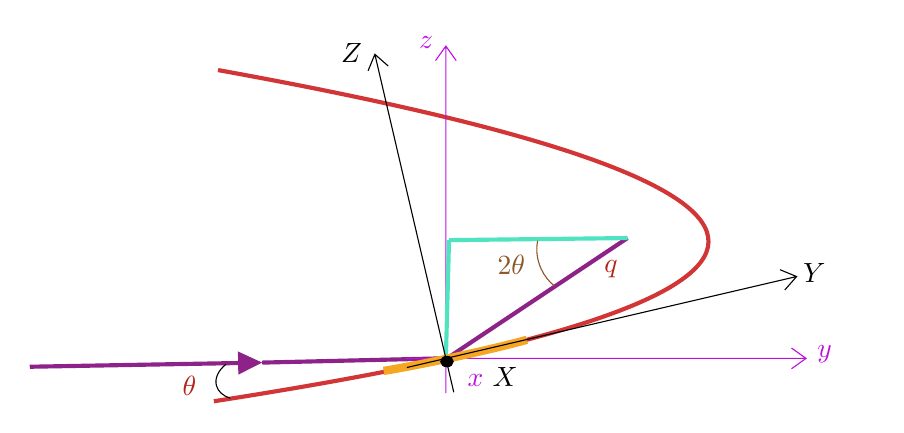
\begin{tikzpicture}[x=0.75pt,y=0.75pt,yscale=-1,xscale=1]
%uncomment if require: \path (0,214); %set diagram left start at 0, and has height of 214

%Shape: Parabola [id:dp636758281566334] 
\draw  [color={rgb, 255:red, 209; green, 53; blue, 53 }  ,draw opacity=1 ][line width=1.5]  (215.73,193.63) .. controls (532.78,144.36) and (533.44,91.17) .. (217.71,34.06) ;
%Straight Lines [id:da5751643928734858] 
\draw [color={rgb, 255:red, 141; green, 34; blue, 137 }  ,draw opacity=1 ][line width=1.5]    (239,175) -- (324,173) ;
%Straight Lines [id:da4985393188459284] 
\draw [color={rgb, 255:red, 141; green, 34; blue, 137 }  ,draw opacity=1 ][line width=1.5]    (328,173) -- (415,115) ;
%Shape: Axis 2D [id:dp5339485321600788] 
\draw [color={rgb, 255:red, 189; green, 16; blue, 224 }  ,draw opacity=1 ] (308.2,172.98) -- (501,172.98)(327.48,22.53) -- (327.48,189.7) (494,167.98) -- (501,172.98) -- (494,177.98) (322.48,29.53) -- (327.48,22.53) -- (332.48,29.53)  ;
%Straight Lines [id:da984423242776999] 
\draw [color={rgb, 255:red, 141; green, 34; blue, 137 }  ,draw opacity=1 ][line width=1.5]    (127,177) -- (235,175.07) ;
\draw [shift={(239,175)}, rotate = 538.98] [fill={rgb, 255:red, 141; green, 34; blue, 137 }  ,fill opacity=1 ][line width=0.08]  [draw opacity=0] (11.61,-5.58) -- (0,0) -- (11.61,5.58) -- cycle    ;
%Straight Lines [id:da25833218941129754] 
\draw [color={rgb, 255:red, 80; green, 227; blue, 194 }  ,draw opacity=1 ][line width=1.5]    (329,116) -- (415,115) ;
%Straight Lines [id:da4020633150416717] 
\draw [color={rgb, 255:red, 80; green, 227; blue, 194 }  ,draw opacity=1 ][line width=1.5]    (329,116) -- (327.48,172.98) ;
%Shape: Arc [id:dp507008334854385] 
\draw  [draw opacity=0] (379.83,138.12) .. controls (377.17,136.02) and (374.91,133.19) .. (373.35,129.77) .. controls (371.31,125.28) and (370.83,120.52) .. (371.71,116.28) -- (389.13,122.59) -- cycle ; \draw  [color={rgb, 255:red, 139; green, 87; blue, 42 }  ,draw opacity=1 ] (379.83,138.12) .. controls (377.17,136.02) and (374.91,133.19) .. (373.35,129.77) .. controls (371.31,125.28) and (370.83,120.52) .. (371.71,116.28) ;
%Shape: Arc [id:dp28668965321519213] 
\draw  [draw opacity=0] (223.6,192.18) .. controls (220.17,191.08) and (217.66,188.93) .. (216.92,186.03) .. controls (216.01,182.5) and (217.91,178.69) .. (221.55,175.8) -- (232.39,182.04) -- cycle ; \draw   (223.6,192.18) .. controls (220.17,191.08) and (217.66,188.93) .. (216.92,186.03) .. controls (216.01,182.5) and (217.91,178.69) .. (221.55,175.8) ;
%Curve Lines [id:da06756156046542072] 
\draw [color={rgb, 255:red, 245; green, 166; blue, 35 }  ,draw opacity=1 ][line width=3]    (297.5,179) .. controls (318.17,175.67) and (355.17,167.33) .. (366.5,164) ;
%Shape: Axis 2D [id:dp06708045637689208] 
\draw [color={rgb, 255:red, 0; green, 0; blue, 0 }  ,draw opacity=1 ] (308.7,177.37) -- (496.46,133.54)(293.28,26.46) -- (331.28,189.26) (488.5,130.26) -- (496.46,133.54) -- (490.78,140) (290,34.42) -- (293.28,26.46) -- (299.74,32.14)  ;
%Shape: Ellipse [id:dp8232202429248765] 
\draw  [fill={rgb, 255:red, 0; green, 0; blue, 0 }  ,fill opacity=1 ] (325,174.5) .. controls (325,173.12) and (326.34,172) .. (328,172) .. controls (329.66,172) and (331,173.12) .. (331,174.5) .. controls (331,175.88) and (329.66,177) .. (328,177) .. controls (326.34,177) and (325,175.88) .. (325,174.5) -- cycle ;

% Text Node
\draw (510,171) node  [color={rgb, 255:red, 179; green, 35; blue, 24 }  ,opacity=1 ,rotate=-359.63]  {$\textcolor[rgb]{0.74,0.06,0.88}{y}$};
% Text Node
\draw (318,21) node  [color={rgb, 255:red, 179; green, 35; blue, 24 }  ,opacity=1 ,rotate=-359.63]  {$\textcolor[rgb]{0.74,0.06,0.88}{z}$};
% Text Node
\draw (282,26) node  [color={rgb, 255:red, 179; green, 35; blue, 24 }  ,opacity=1 ,rotate=-359.63]  {$\textcolor[rgb]{0,0,0}{Z}$};
% Text Node
\draw (505,132) node  [color={rgb, 255:red, 179; green, 35; blue, 24 }  ,opacity=1 ,rotate=-359.63]  {$\textcolor[rgb]{0,0,0}{Y}$};
% Text Node
\draw (350,182) node  [color={rgb, 255:red, 179; green, 35; blue, 24 }  ,opacity=1 ,rotate=-359.63]  {$\textcolor[rgb]{0.74,0.06,0.88}{x} \ \textcolor[rgb]{0,0,0}{X}$};
% Text Node
\draw (407,130) node  [color={rgb, 255:red, 179; green, 35; blue, 24 }  ,opacity=1 ,rotate=-359.63]  {$q$};
% Text Node
\draw (204,186) node  [color={rgb, 255:red, 179; green, 35; blue, 24 }  ,opacity=1 ,rotate=-359.63]  {$\theta $};
% Text Node
\draw (359,128) node  [color={rgb, 255:red, 139; green, 87; blue, 42 }  ,opacity=1 ,rotate=-359.63]  {$2\theta $};


\end{tikzpicture}




\end{figure}

%%%%%%%%%%%%%%%%%%%%%%%%%%%%%%%%  end put here figure %%%%%%%%%%%%%%%%%%%%%%%%%%%%%%%%%%%%%%%%%%%%%%%%

\end{document}




\caption{Schematic (vertical section) of the reference frames: mirror-related $(X,Y,Z)$ used for numerical implementation, and mirror-canonical $(x,y,z)$ where the diaboloid shape takes the form of Eq.~\ref{eqn:diaboloidV}. \todo{A 3D VIEW AND MAY BE A SAGITTAL SECTION COULD BE ADDED}}
\end{figure}



The equation of the diaboloid in the ``collimaing'' configuration takes the form  Ref.~\cite{valSPIE} 
\todo{IT MAY BE DEDUCED IN AN APPENDIX OR SUPPLEMENTARY MATERIAL FOLLOWING KEN LSBL1440 AND HOWARD LSBL 1465 FOR THE ELLIPSE}

\begin{multline}
\label{eqn:diaboloidV}
z(x,y) = q \sin2\theta - 
[ (q \sin{2\theta})^2 + 2p^2 + 2 p q + \\
2 (p + q \cos{2\theta}) y - 
2 (p+q)  \sqrt{x^2 + (y + p)^2}) 
]^{1/2}.
\end{multline}
The mirror height is $z$=0 at the mirror center position $x, y$=0, as expected. The tangential profile ($x$=0) is a parabola $y=q \sin2\theta + z^2/(4f)$ and focal length $ f = q (1-\cos2\theta) /2$. For small angles ($\cos2\theta\approx 1 - 2\theta^2$) and $|y|\ll q$ gives $z\approx 2 \theta q + \theta y$ with slope in the center $dz/dy=\theta$. The sagittal section ($y$=0) is an ellipse $x^2/a^2 + (z + q \sin2\theta)^2/b^2=1$ with semiaxes $a=q \sin2\theta$ and $b=a \sqrt{p /(p+q)}$. 

For ray tracing calculations it is convinient to obtain the numerical mesh as a function of a mirror-related coordinate system ($X,Y,Z$) (Fig.~\ref{fig:frame}), with origin in the center of the mirror, one axis ($Y$) tangent to the diaboloid surface origin in the direction of the beam propagation, another axis ($X$) tangent to the diaboloid surface origin in the direction perpendicular of the beam propagation, and the third axis ($Z$) is outward pointing perpendicular to $X$ and $Y$. \inred{Therefore the surface in its explicit form needed for being evaluated numerically is $Z(X,Y)$ with $X \in [-W/2, W/2]$ and $Y \in [-L/2, L/2]$ with $L$ the mirror length and $W$ the mirror width. The mirror length is sampled in $N_Y$ points and the mirror width in $N_X$ points, therefore the height or elevation of a point is $Z_{i,j}=Z(X_i,Y_j)$ REMOVE?.}
In most practical cases the grazing incidence $\theta$ is small, therefore Eq.~\ref{eqn:diaboloidV} can be expressed in the $X,Y,Z$ frame by forcing zero slope at the origin (i.e., detrending the plane $z_{plane}=y \theta$). This is done numerically after evaluating the surface using Eq.~\ref{eqn:diaboloidV}. 
The exact explicit expression of the diaboloid $Z(X,Y)$ can be obtained from the rotation of Eq.~\ref{eqn:diaboloidV} an angle $\theta$ \cite{part2}, resulting in a fourth-degree poynomial equation $F(X,Y,Z)=0$. The explicit equation is therefore obtained by solving this equation for the any point of the $(X_i,Y_j)$ mesh.

The simplest approximaton of the diaboloid is the toroid, approximated by a doubly bent surface with radii $R_m$ and $R_s$ (in the meridional and sagittal directions, respectively) given by the focusing conditions (Coddington equations):

\begin{equation}
\label{eqn:radii}
\frac{1}{p} = \frac{2 }{R_m \sin\theta };~~~~~~
\frac{1}{p} + \frac{1}{q} = \frac{2\sin\theta}{ R_s}.
\end{equation}

An approximation to the diaboloid is a parabolic cone, in which the tangential shape at a transverse coordinate of zero is the parabola, and the sagittal shape is a circle, whose radius changes as a function of longitudinal coordinate $Y$ \cite{part2}

\begin{multline}
\label{eq:sagRadius}
R_s(Y) 
% = \frac{2  p \sin\theta \cos\theta}{p + q} (q - Y \cos\theta)   \sqrt{Y \cos\theta / p + \cos^2\theta} \\
\approx 
\frac{2p q \cos^2\theta \sin\theta  }{p + q} - 
\frac{\cos\theta \sin\theta (2 p \cos^2\theta - q)}{p + q} Y.
\end{multline}
The central sagittal radius $R_s(Y=0)=p q \sin\theta \cos^2\theta/ (p+q)$ is very close, but not exact to the one given by the Coddington equation $R_s^c=2 p q \sin\theta / (p+q)$.


\subsection{Numerical implementation and testing}
\label{sec:oasys}

A graphical interface or widget in the Oasys environment  creates the diaboloid surface and its approximations in the form of a numerical mesh. The user selects the type of surface to calculate (diaboloid or other approximations), the mirror geometry (size and sampling) and the focusing arrangement (conversion from cylindrical to spherical wave or viceversa). 
The diaboloid is implemented in an approximated way by using the detrended Eq.\ref{eqn:diaboloidV} or in an exact form by solving numerically its implicit quartic equation using the {\tt fqs} python library by N. Krvavika ({\tt https://github.com/NKrvavica/fqs}). 
The interface also allows to remove the toroid from the calculated surface to visualize and use the aspherical components. The surface is written in a {\tt hdf5} formatted file, as it is standard for Oasys surfaces. This format allows to input easily the numerical surface into several Oasys applications, like the ray tracing tool ShadowOui \cite{codeSHADOWOUI}, but also in wave-optics codes. A view of the interface is in Fig.~\ref{fig:widget}.

\begin{figure}\label{fig:widget}
\centering
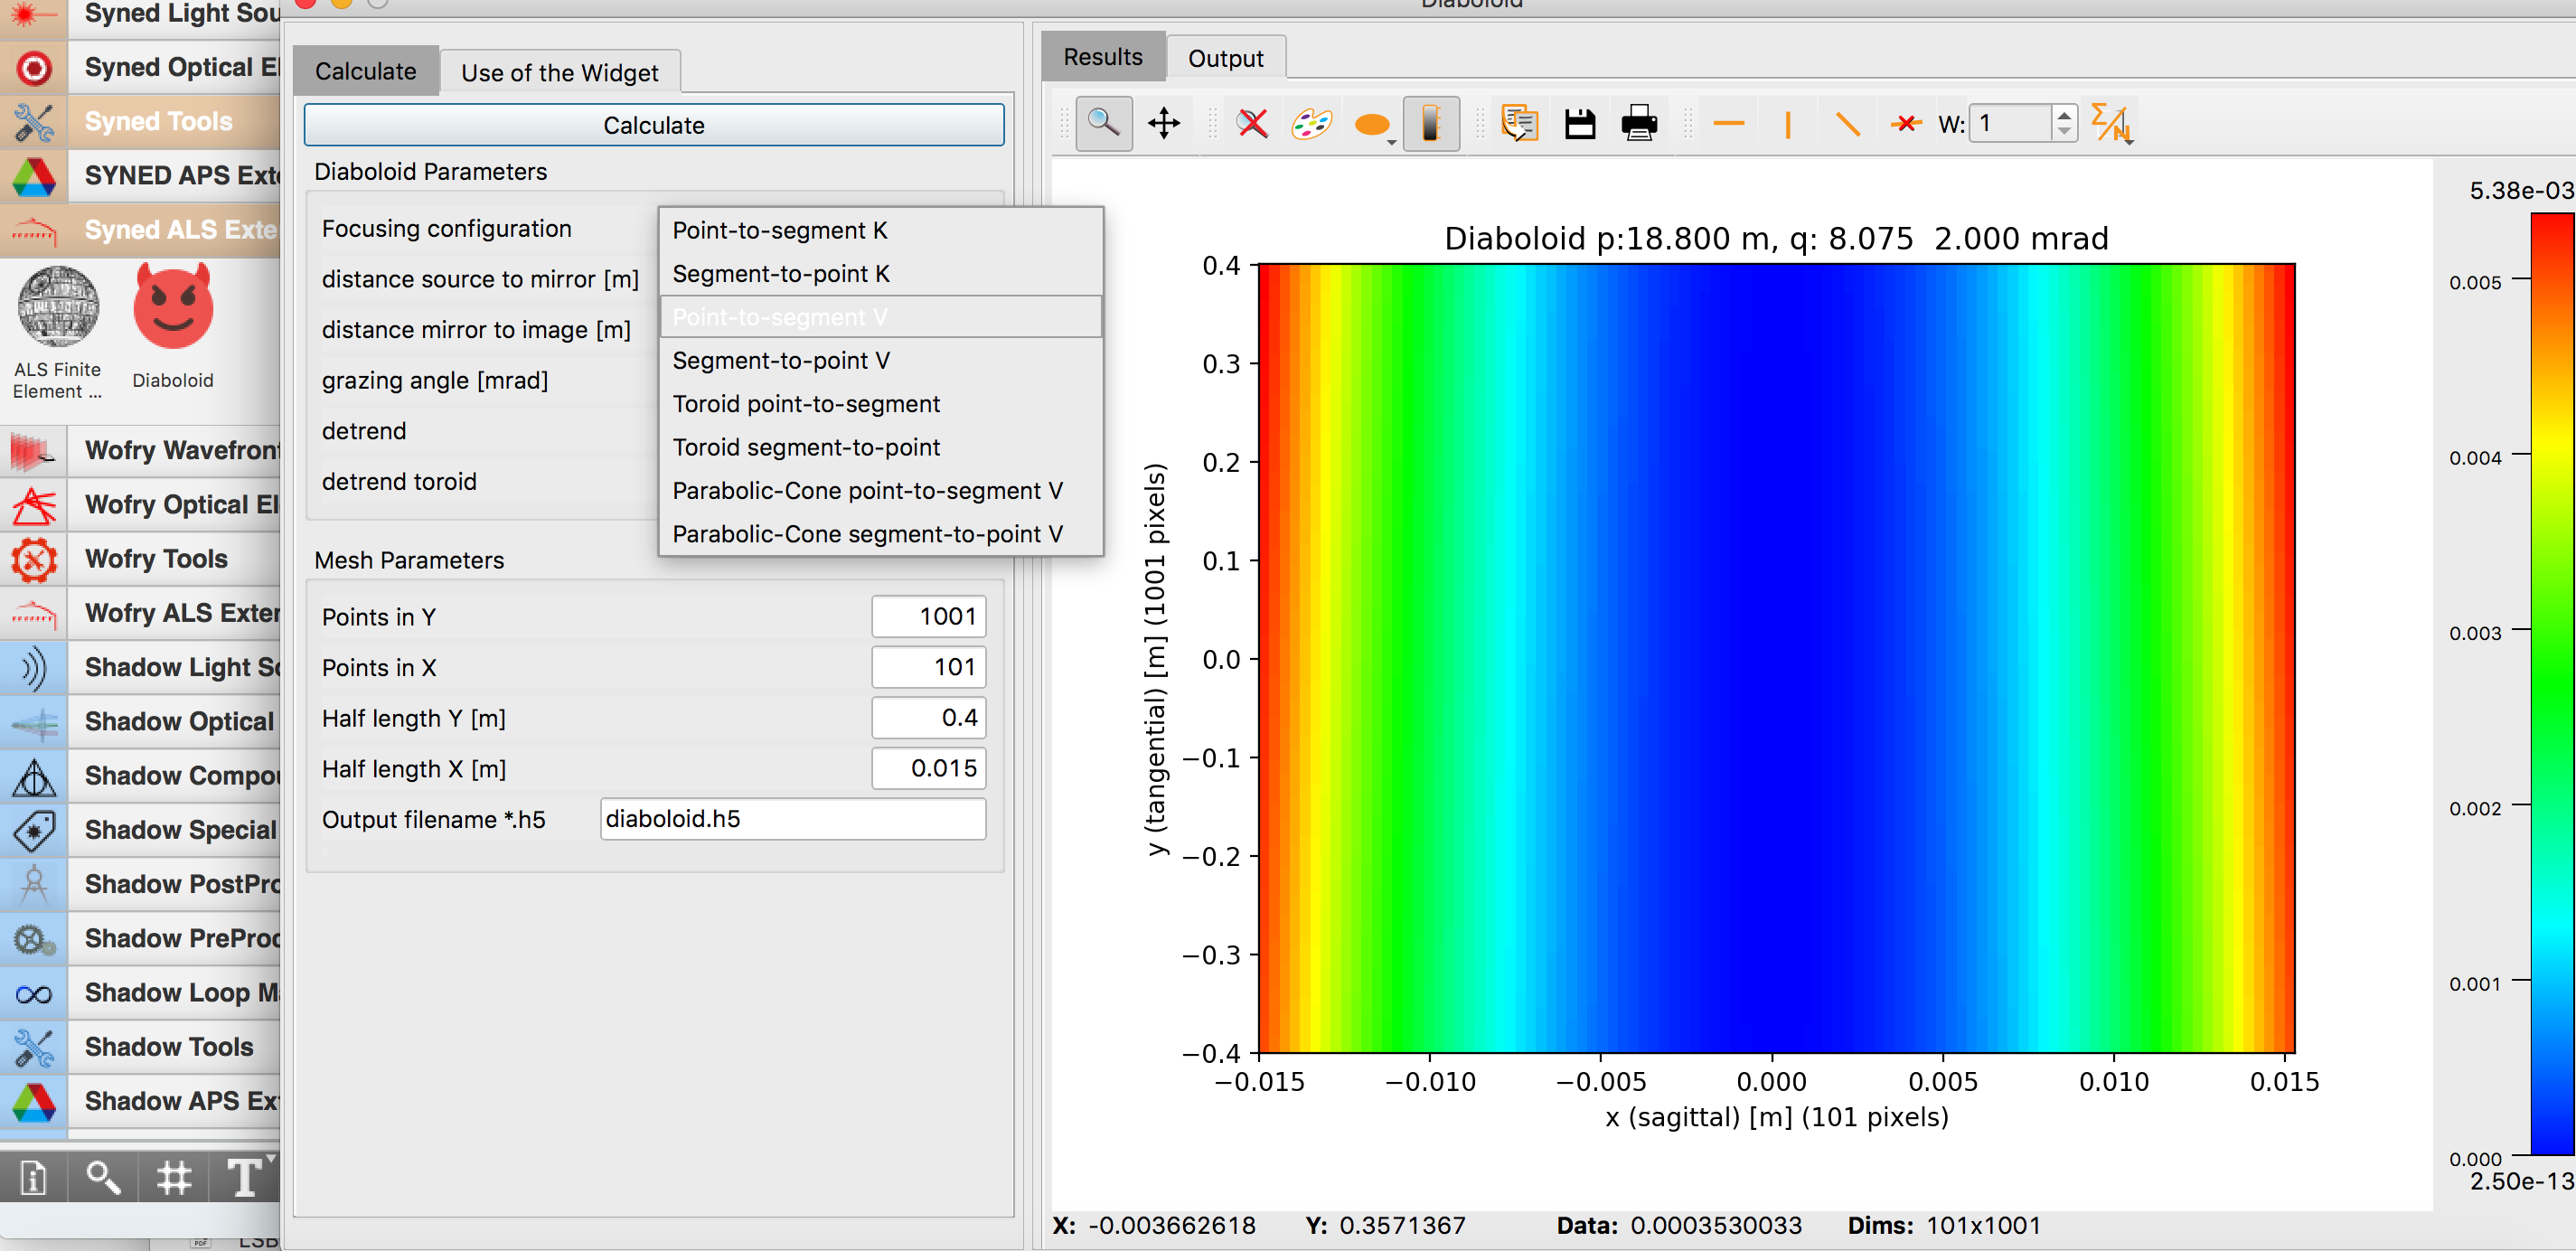
\includegraphics[width=0.95\textwidth]{figures/widget.png}
\caption{View of the interface to create the numerical sampling of the diaboloid and related surfaces ("Diaboloid" widget in Oasys/Syned) }
\end{figure}


We performed ray tracing using a single diaboloid with the purpose to test the accuracy of the calculations. The simpler case of point-to-segment configuration is chosen, with $p$=29.3~m, $q$=19.53~m and $\theta$=4.5~mrad. A point source is created with divergence large enough to fully illuminate the mirror dimensions: length $L$=0.2~m, and width $W$=0.02~m.

\begin{figure}\label{fig:pointToSegment}
\flushleft
~~~~~~a)~~~~~~~~~~~~~~~~~~~~~~~~~~~~~~~~~~~~~~~~~~~~b)\\
\centering
% 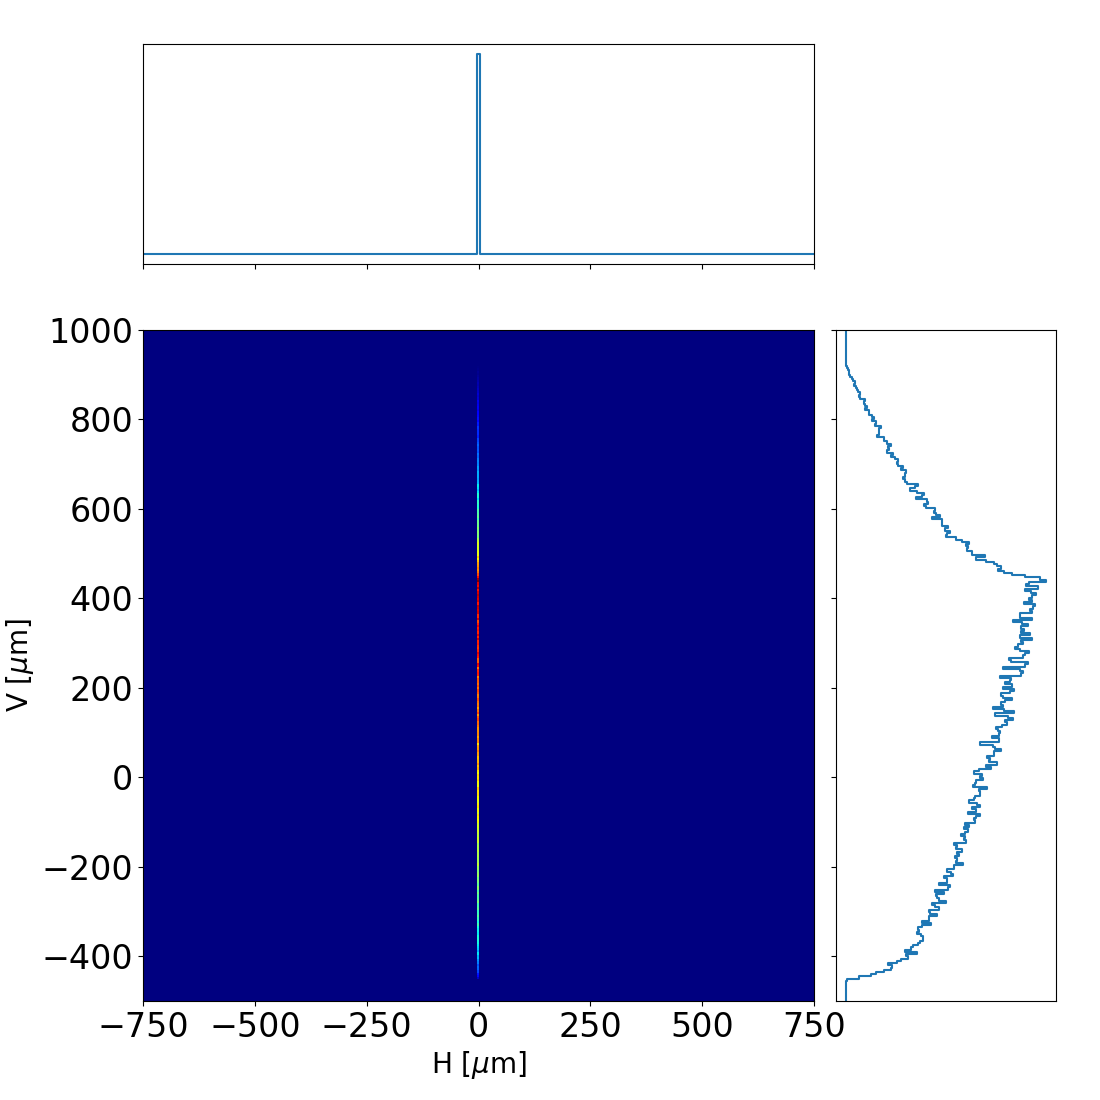
\includegraphics[width=0.22\textwidth]{figures/p2s_V.png}
% 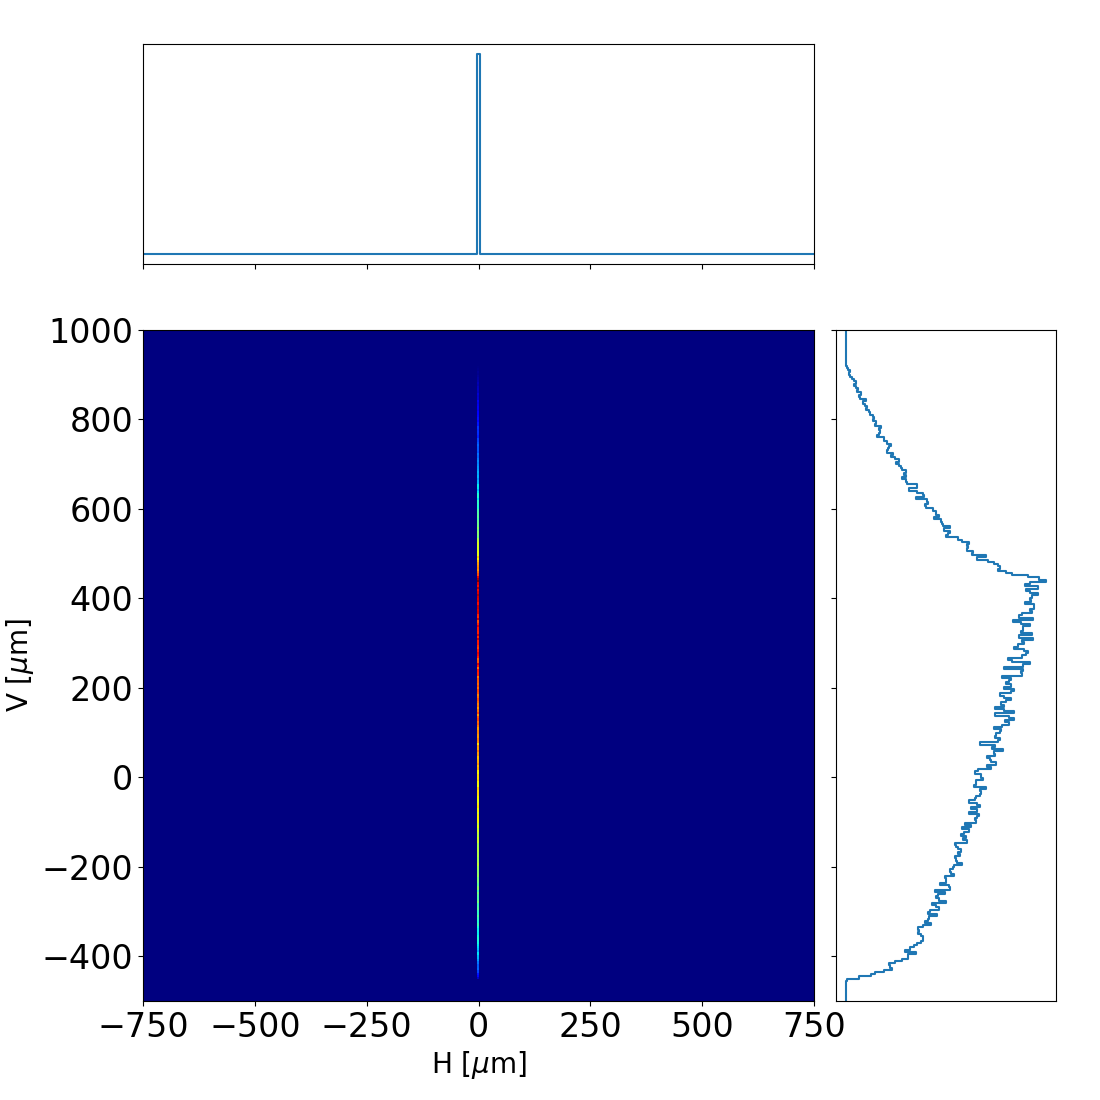
\includegraphics[width=0.22\textwidth]{figures/p2s_K.png}
% 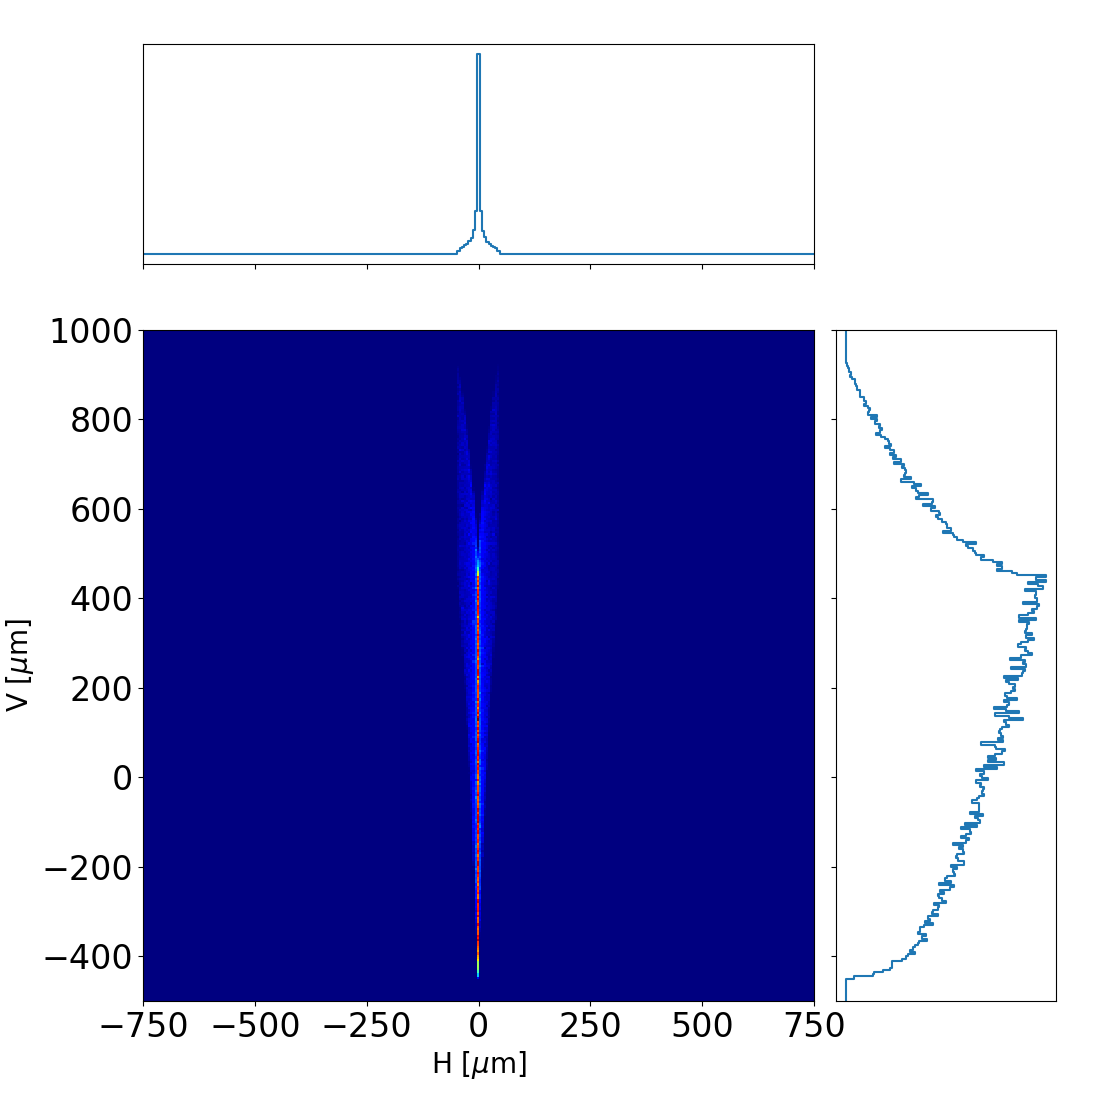
\includegraphics[width=0.22\textwidth]{figures/p2s_parabolic-cone.png}
% 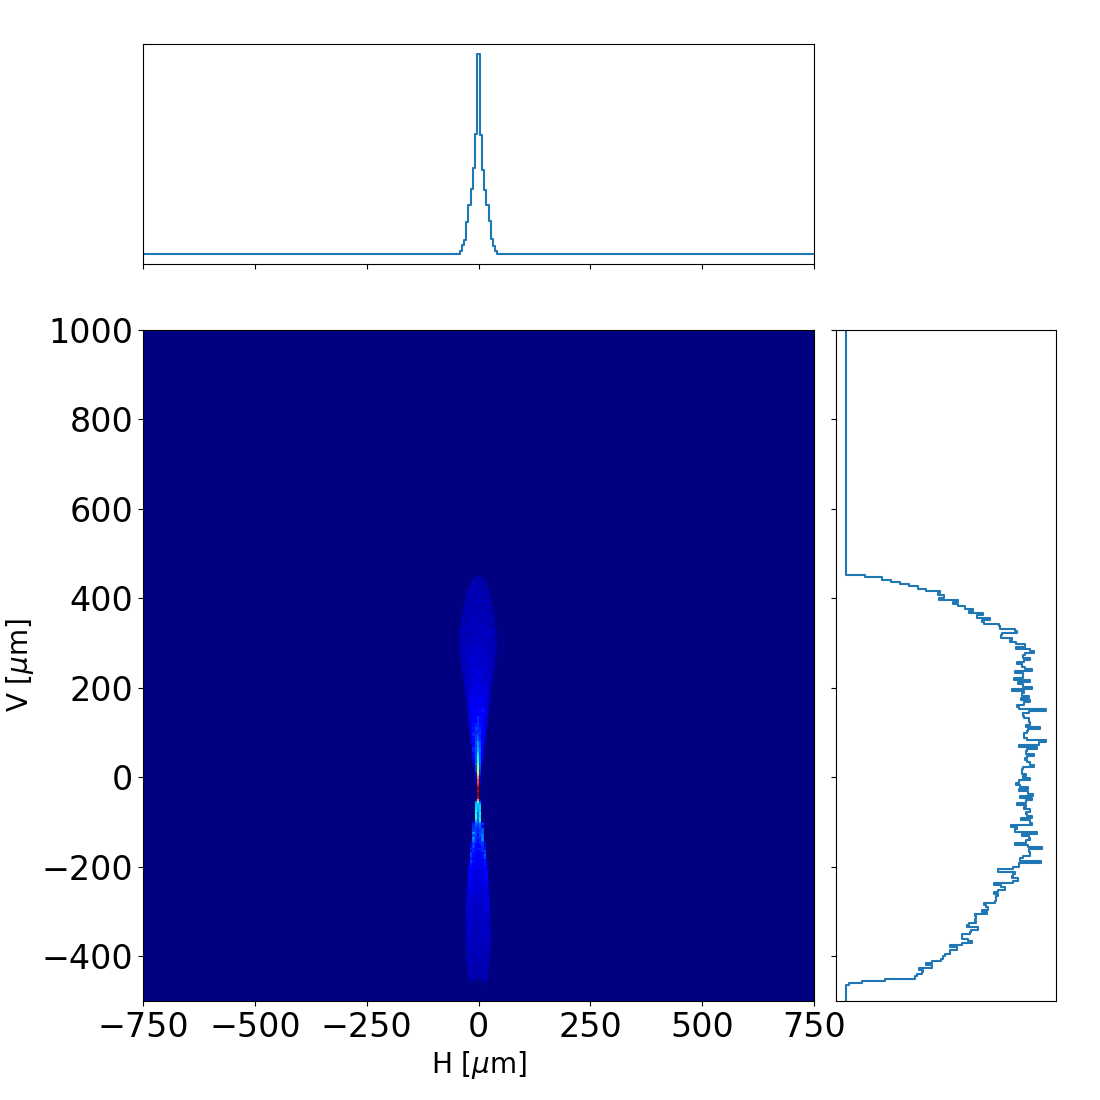
\includegraphics[width=0.22\textwidth]{figures/p2s_toroid.png}

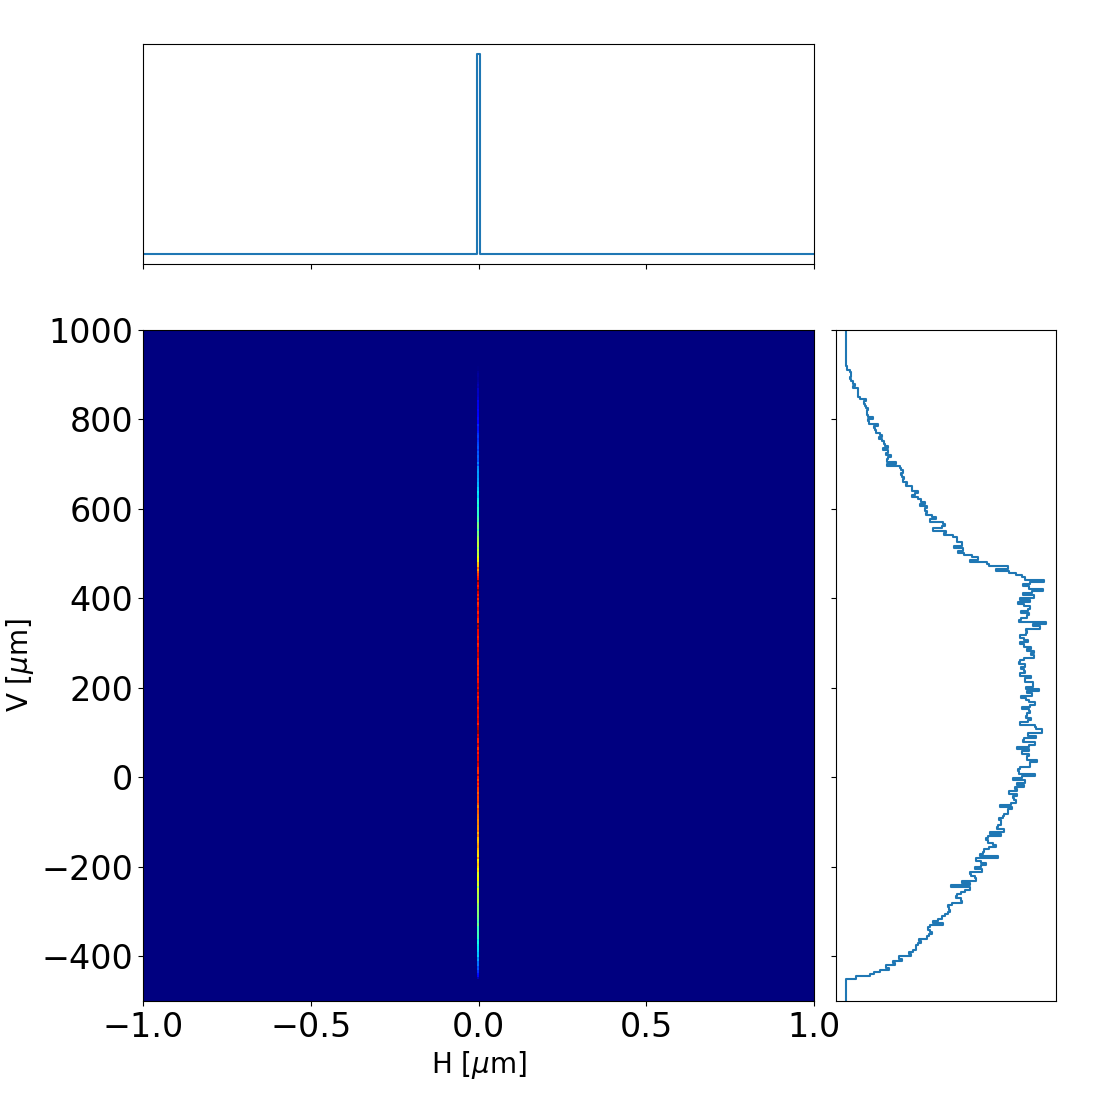
\includegraphics[width=0.49\textwidth]{figures/p2s_V_z.png}
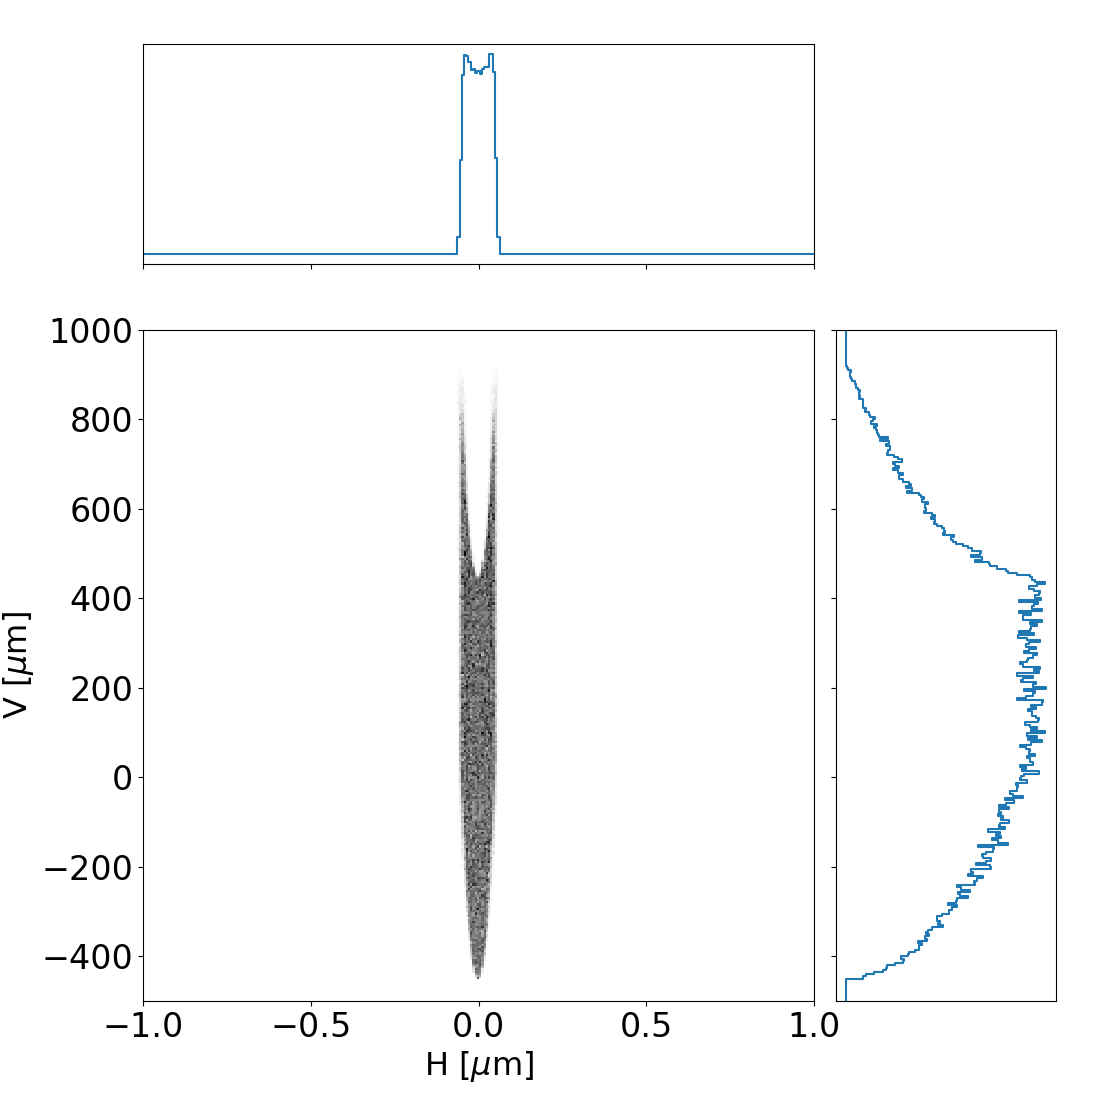
\includegraphics[width=0.49\textwidth]{figures/p2s_K_z.png} \\
\flushleft
% ~~~~~~c)~~~~~~~~~~~~~~~~~~~~~~~~~~~~~~~~~~~~~~~~~d)\\
% 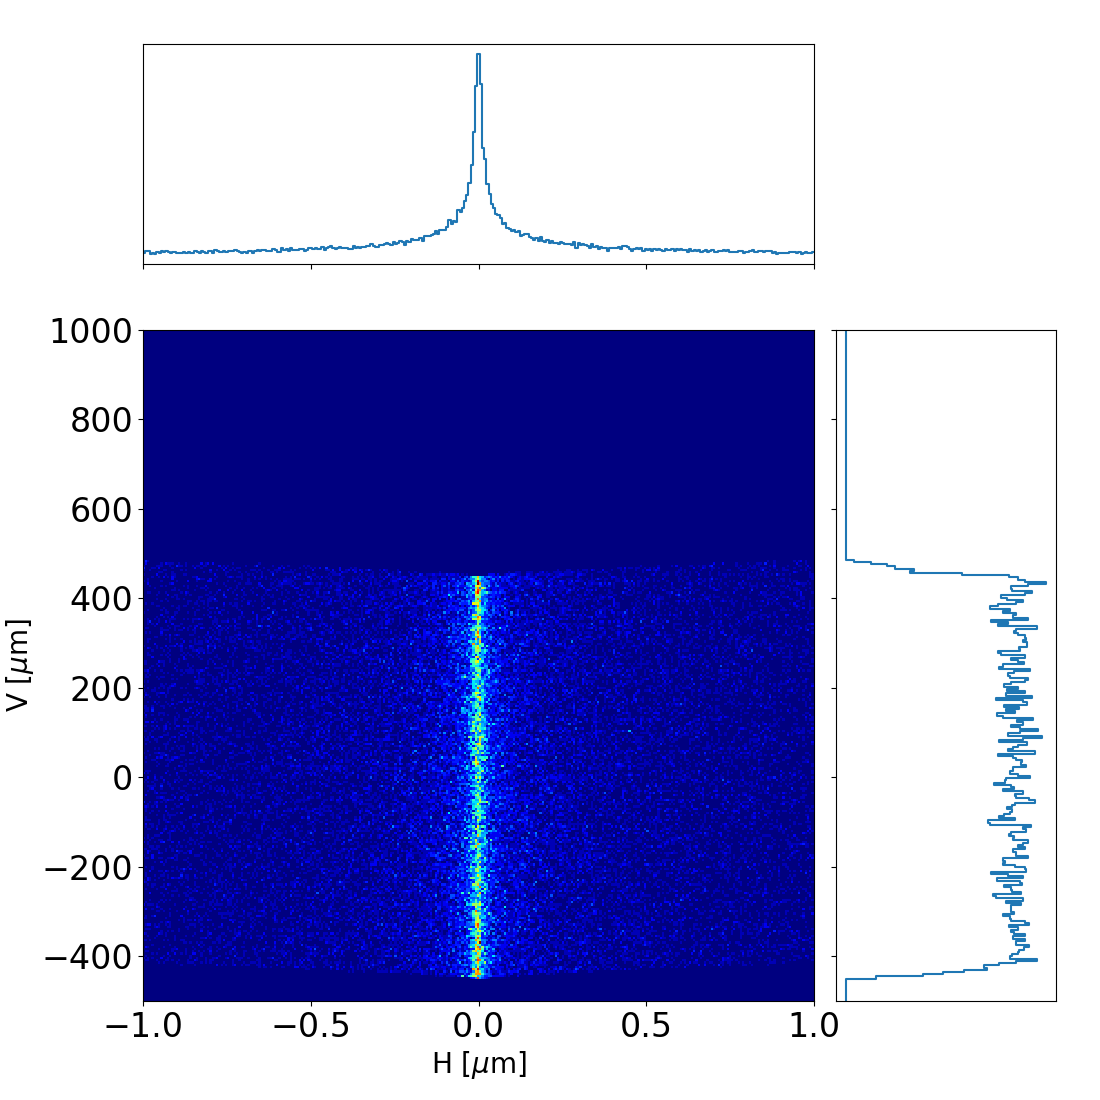
\includegraphics[width=0.49\textwidth]{figures/p2s_parabolic-cone_z.png}
% 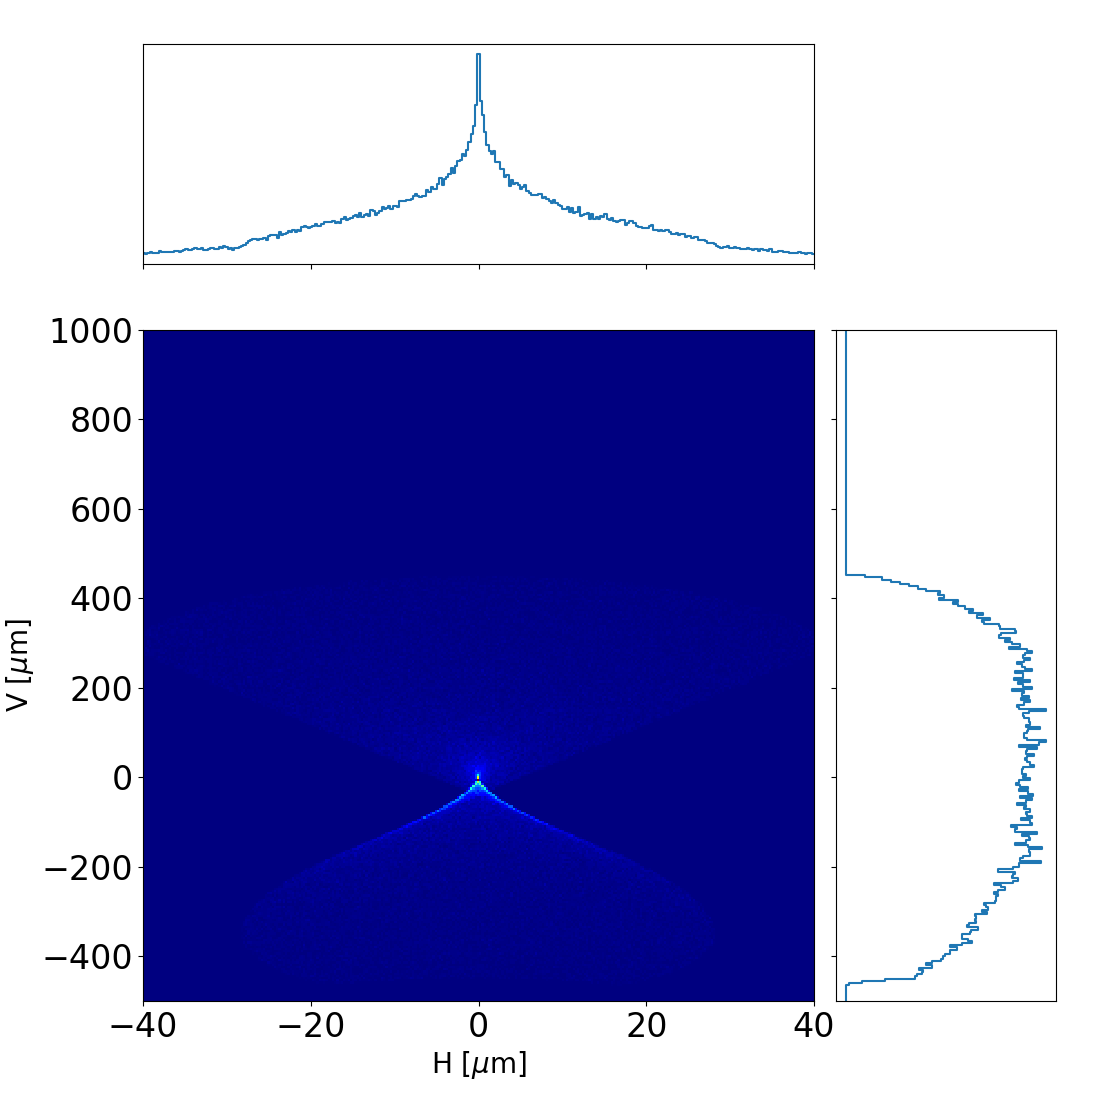
\includegraphics[width=0.49\textwidth]{figures/p2s_toroid_z.png}
\caption{Comparison of images produced by a diaboloid surface focusing in horizontal and collimating in vertical using different implementations: a) diaboloid exact implementation (solving quartic equation),and b) diaboloid approximated implementation (Eq.~\ref{eqn:diaboloidV} detrended with $z_{plane}=\theta Y$).
%, c) parabolic-quasicone (Eq.~\ref{eqn:parabolicCone}) and d) toroid. Note the different scales in horizontal and vertical. 
The Full-Width at Half-Maximum (FWHM) is 0.3 nm (a) and 93 nm (b). %, 22 nm (c), and 2.5 $\mu$m (d).
}
\end{figure}

The expected result at the focal position is a line focus (segment) with zero dimension in horizontal and a length of $L\sin\theta$ in vertical. The ray tracing results are shown in Fig.~\ref{fig:pointToSegment} where the focal images produced by a diaboloid calculated with the two mentioned methods (exact diaboloid and detrended Eq.~\ref{eqn:diaboloidV}).
The intensity profile along the vertical direction has a non-uniform profile due to the beam intensity projected on the mirror surface with a grazing angle.
%As expected, the toroid produces a very aberrated and wide spot (2.5 $\mu$m FWHM and high tails). The parabolic-quasicone reduces the FWHM by two orders of magnitude (22 nm). Aberration tails are observed in this case. 
Both numerical surfaces produce an almost perfect horizontal focus without aberration tails. However, some residual width is found: 0.3 nm for the exact diaboloid equation and 93 nm for the approximated one. 
%These values are much below the typical dimensions in practical cases where spots of $\mu$m size or larger are expected because the source size and optical aberrations. 
The residual 0.3 nm in the exact implementation is certainly due to numerical rounding errors and also the use of iterative algorithms to find ray intersects, as done in SHADOW.
The approximate form of the diaboloid gives a residual of 93 nm that is mainly originated by the use of the basal plane detrending replacing the exact rotation. It appears, however, to be adequate for all practical implementations, as typically we will be imaging a source with a horizontal size of 10 – 50 microns, and the errors in comparison are insignificant. The approximate method is interesting as it gives an intuitive and simple direct way to visualize the surface.

\section{Ray tracing the ALS beamline 12.2.2}
\label{sec:beamline}

We analyze here the possible use of a diaboloid in a real beamline. We study the case of beamline 12.2.2  at ALS \cite{bl1222} \cite{MacDowell2004}. The source of this beamline is a bending magnet, and we simulated the emission at a photon energy of $E$=30~keV. We consider three cases: i) using a source point, ii) the ALS ring
$\sigma_x$ = 26 $\mu$m, $\sigma_y$ = 10 $\mu$m, electron energy $E_e$=1.9 GeV, magnetic field $B$=5.28~T, and iii) the ALS-U ring, with $\sigma_x$ = 10 $\mu$m, $\sigma_y$ = 7 $\mu$m, $E_e$=2.0~GeV, and $B$=3.1~T. We simulated the combined focusing effect of the two beamline mirrors: M1, a plane parabola placed at $p_1$=6.5~m from the source ($L$ = 900~mm, $\theta$=2 ~mrad); and M2, a refocusing mirror at $p_2$=18.8~m from the source ($L$=800~mm, $W$=20~mm, $\theta$ = 2~mrad. The M2 mirror currently in use is a toroid, which is compared with a possible upgrade with a diaboloid. The exit slit (focal plane) is at $D$=26.875~m from the source.  The M2 magnification M= $(D-p_2)/p_2$=0.43 is close but not exactly matching the "golden" 1:2 toroid geometry \cite{MacDowell2004}. This beamline uses M1 to collimate the beam in the vertical direction in order to optimize the monochromator performance (not simulated) and then 
M2 refocuses the source to the focus from infinity in the vertical direction and the real source in the horizontal direction.

% \begin{figure}\label{fig:bl}
% \centering
% \flushleft
% ~~~~~a)~~~~~~~~~~~~~~~~~~~~~~~~~~~~~~~~~~~~~~~~~~~~~b) \\
% 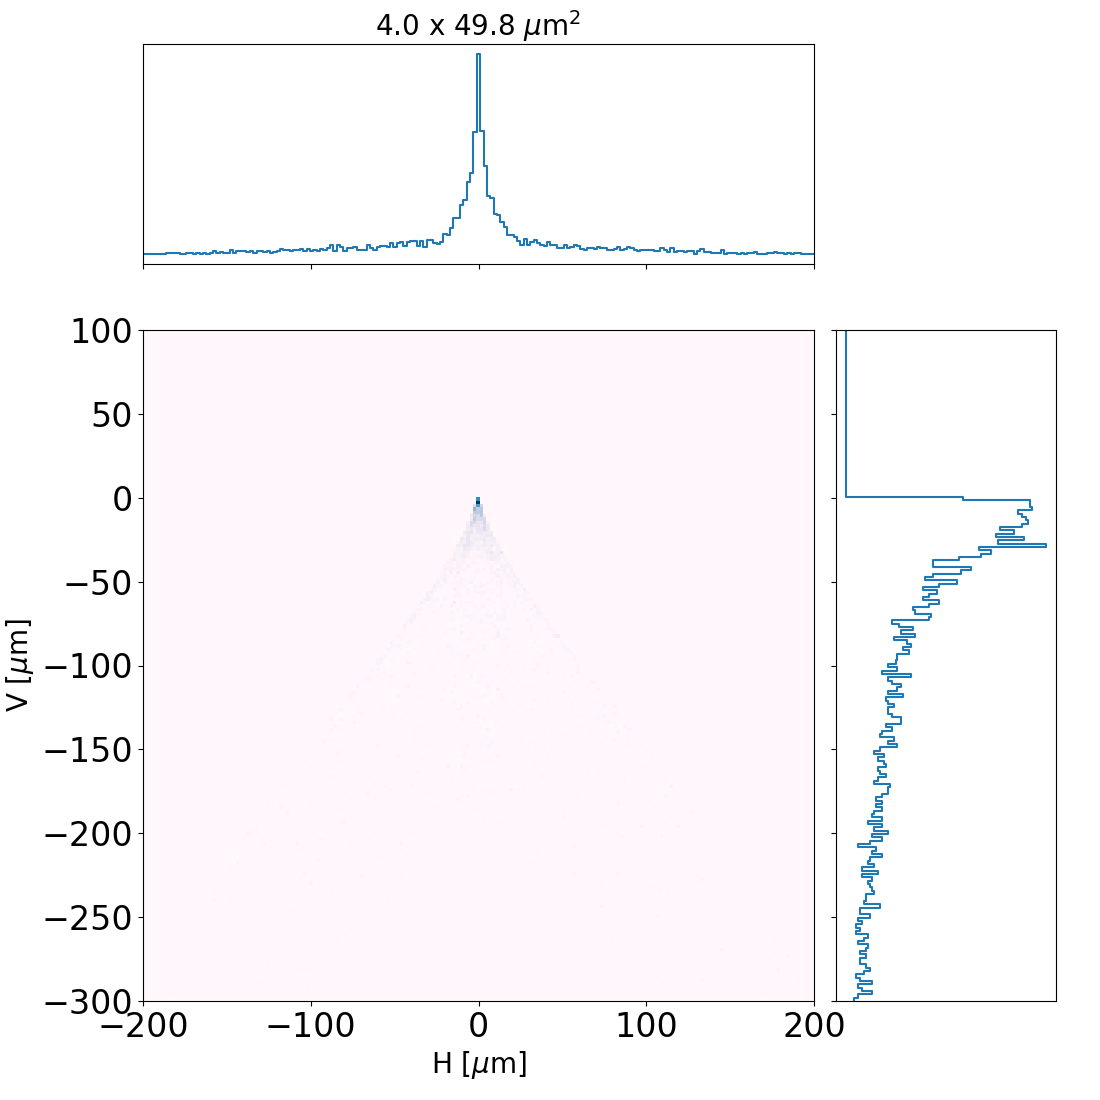
\includegraphics[width=0.45\textwidth]{figures/bl_point_toroid.png} 
% 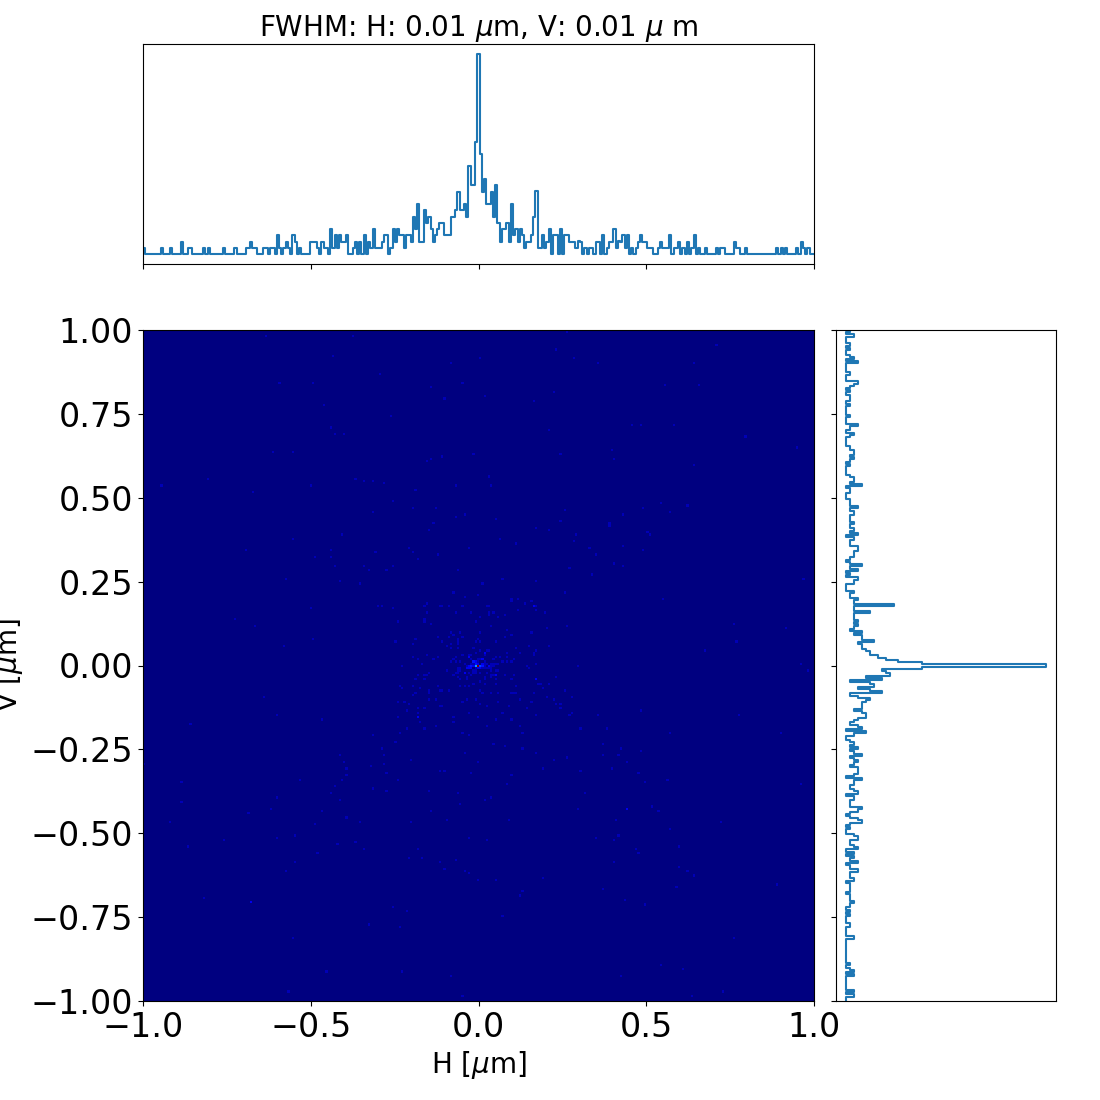
\includegraphics[width=0.45\textwidth]{figures/bl_point_parabolic-cone.png} \\
% \flushleft
% ~~~~~c)~~~~~~~~~~~~~~~~~~~~~~~~~~~~~~~~~~~~~~~~~~~~~d) \\
% 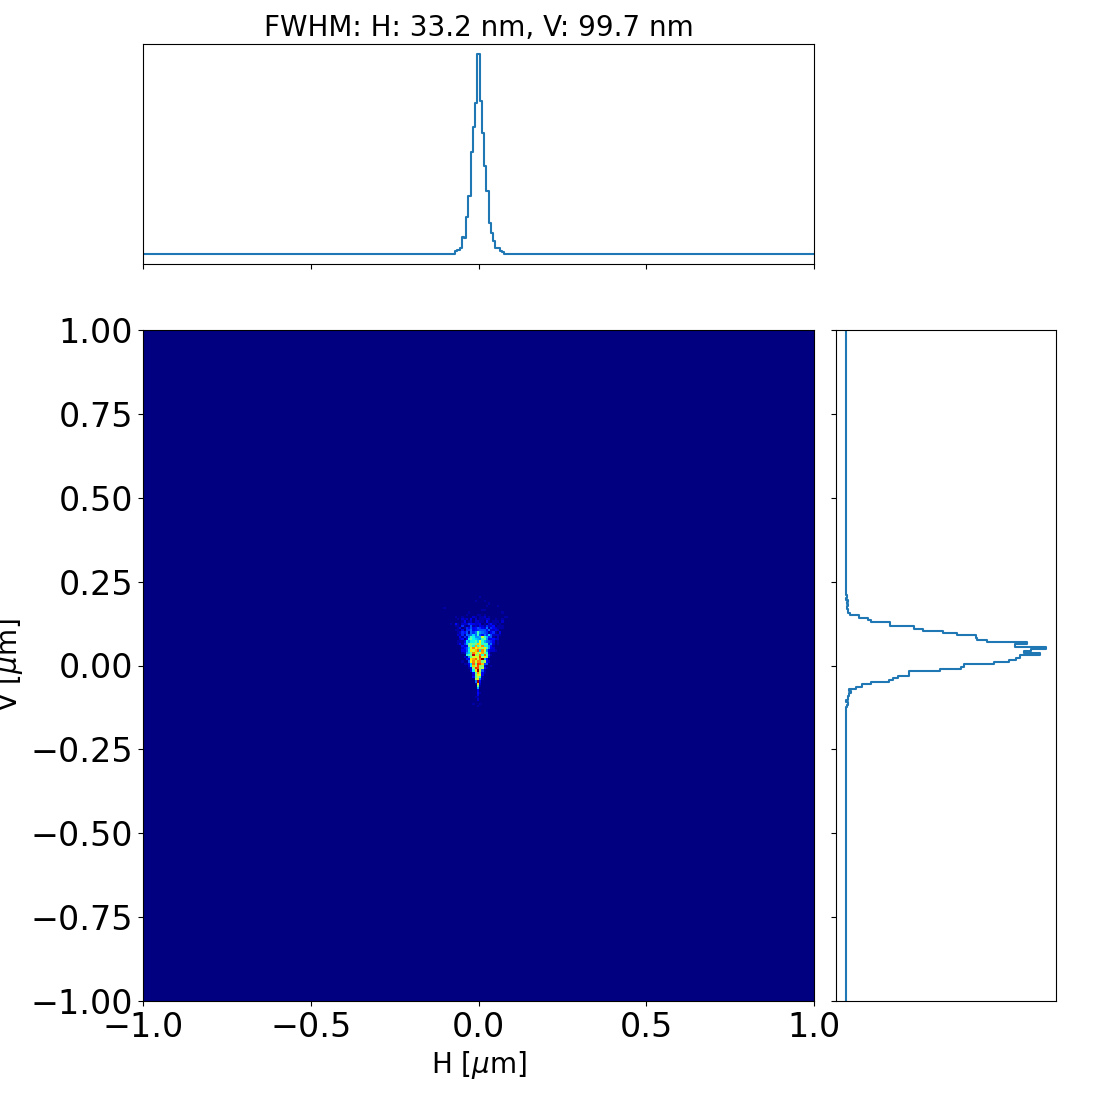
\includegraphics[width=0.45\textwidth]{figures/bl_point_diaboloid.png}
% 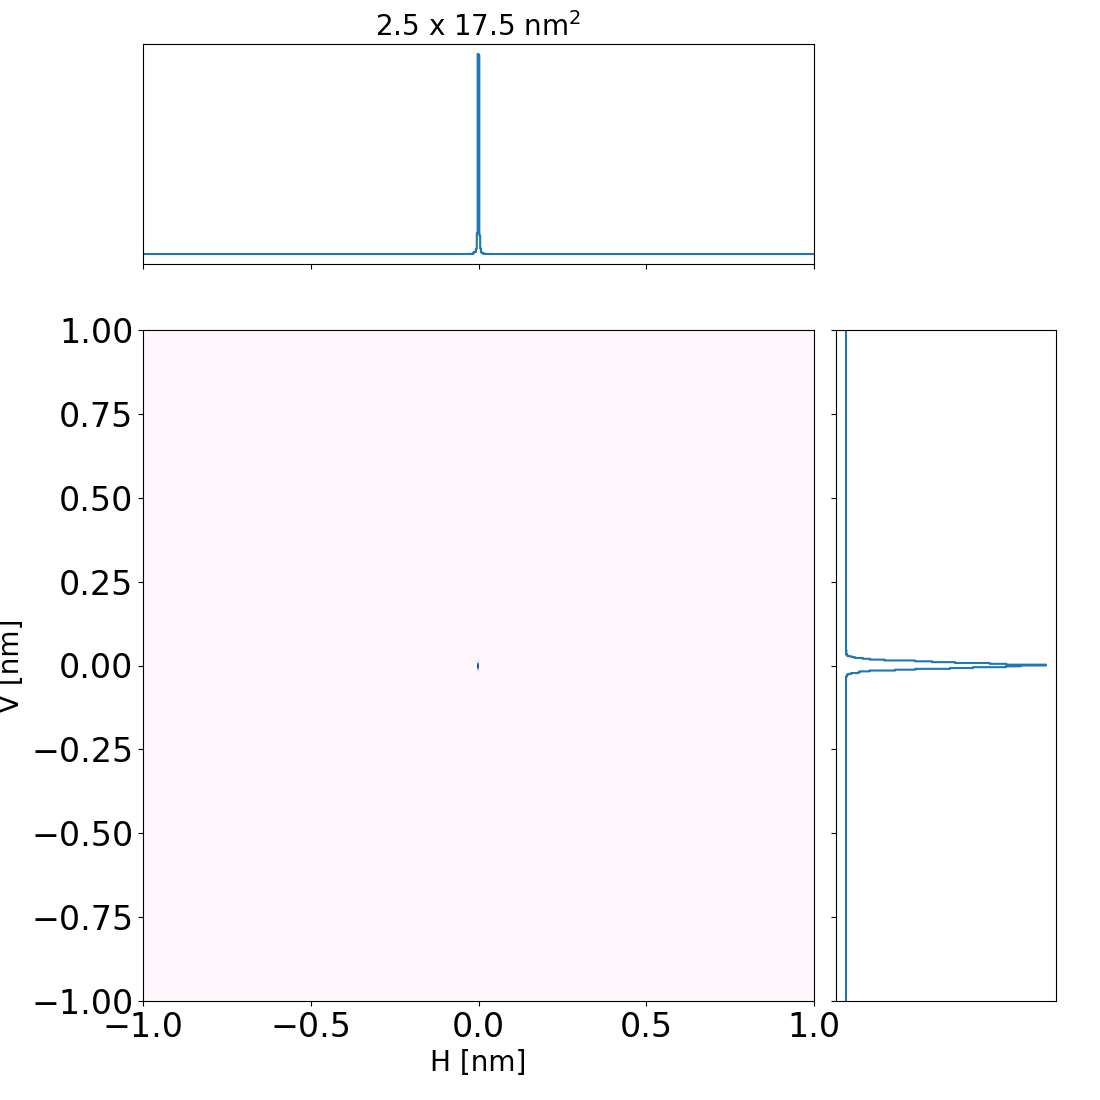
\includegraphics[width=0.45\textwidth]{figures/bl_point_diaboloid-exact.png}
% \caption{Focal image produced by a system of two mirrors M1 (collimating parabola) and M2 represented by (a) a toroid, (b) a parabolic-cone, (c) a diaboloid. The FWHM of the horizontal and vertical histograms are given in the plot titles. The scale changes in the different plots. Note the large size given by the toroid (3 $\times$ 45 $\mu$m$^2$) contrary to all the other surfaces (submicron level)
% }
% \end{figure}

%Figure~\ref{fig:bl} shows a source point imaged by the beamline using for M2 a toroid, a parabolic-cone and a diaboloid. 

\begin{figure}\label{fig:als}
\flushleft
~~~~~a$_1$)~~~~~~~~~~~~~~~~~~~~~~~~~~~~~~~~~~~~~~~~~~~~~b$_1$) \\
\centering
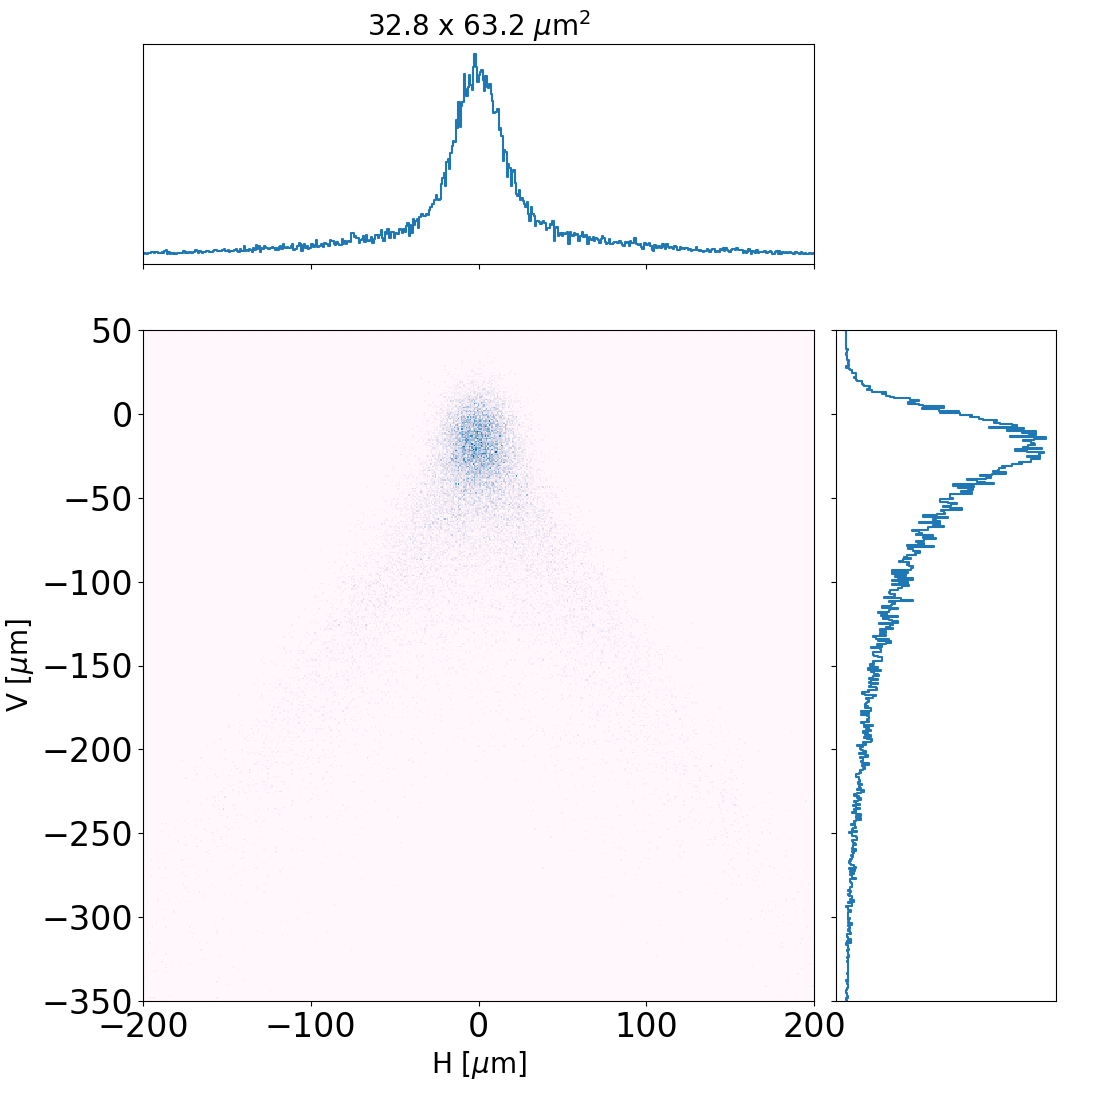
\includegraphics[width=0.45\textwidth]{figures/als_toroid.png}
% 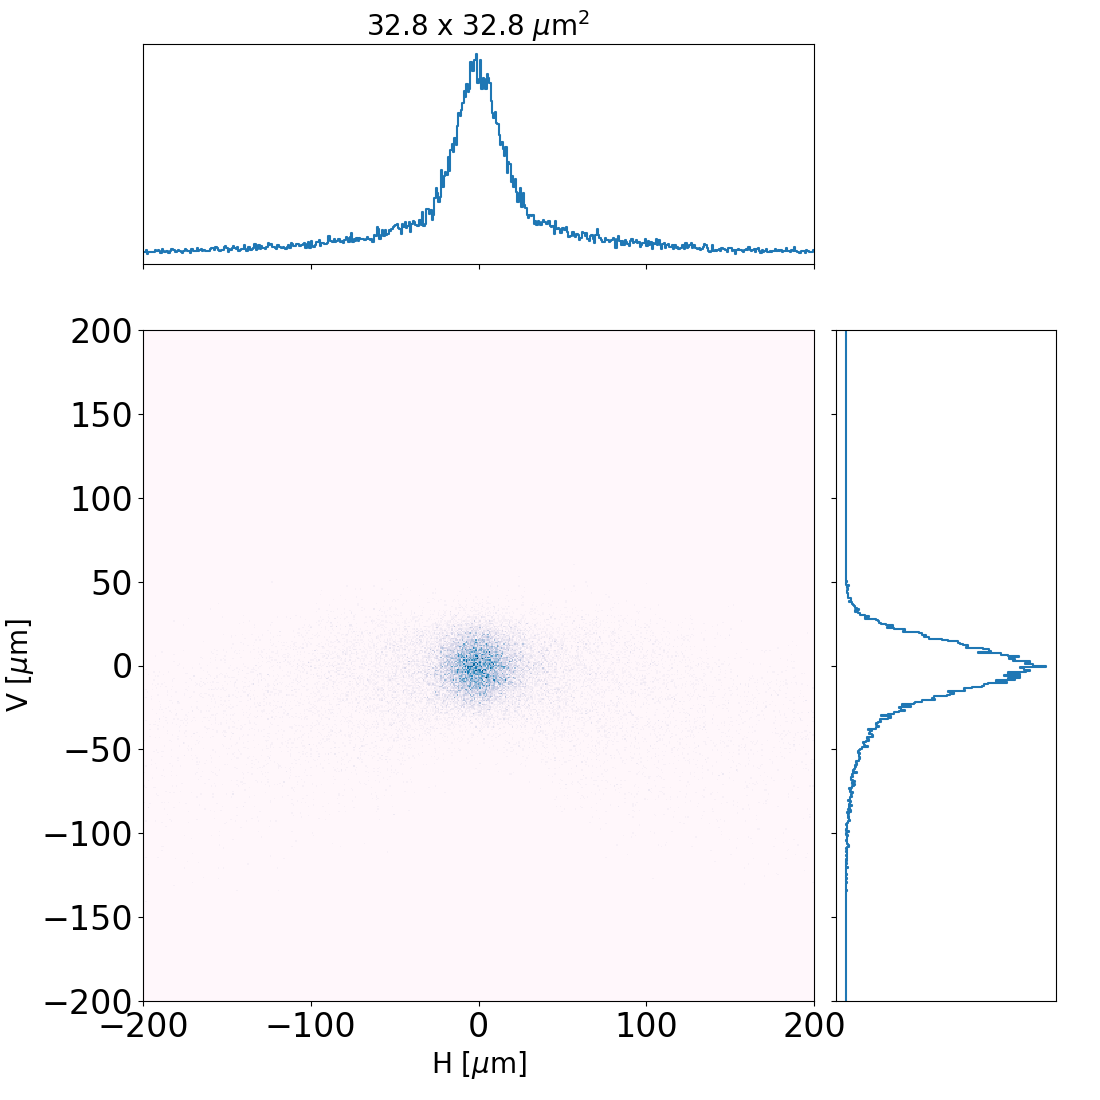
\includegraphics[width=0.32\textwidth]{figures/als_parabolic-cone.png}
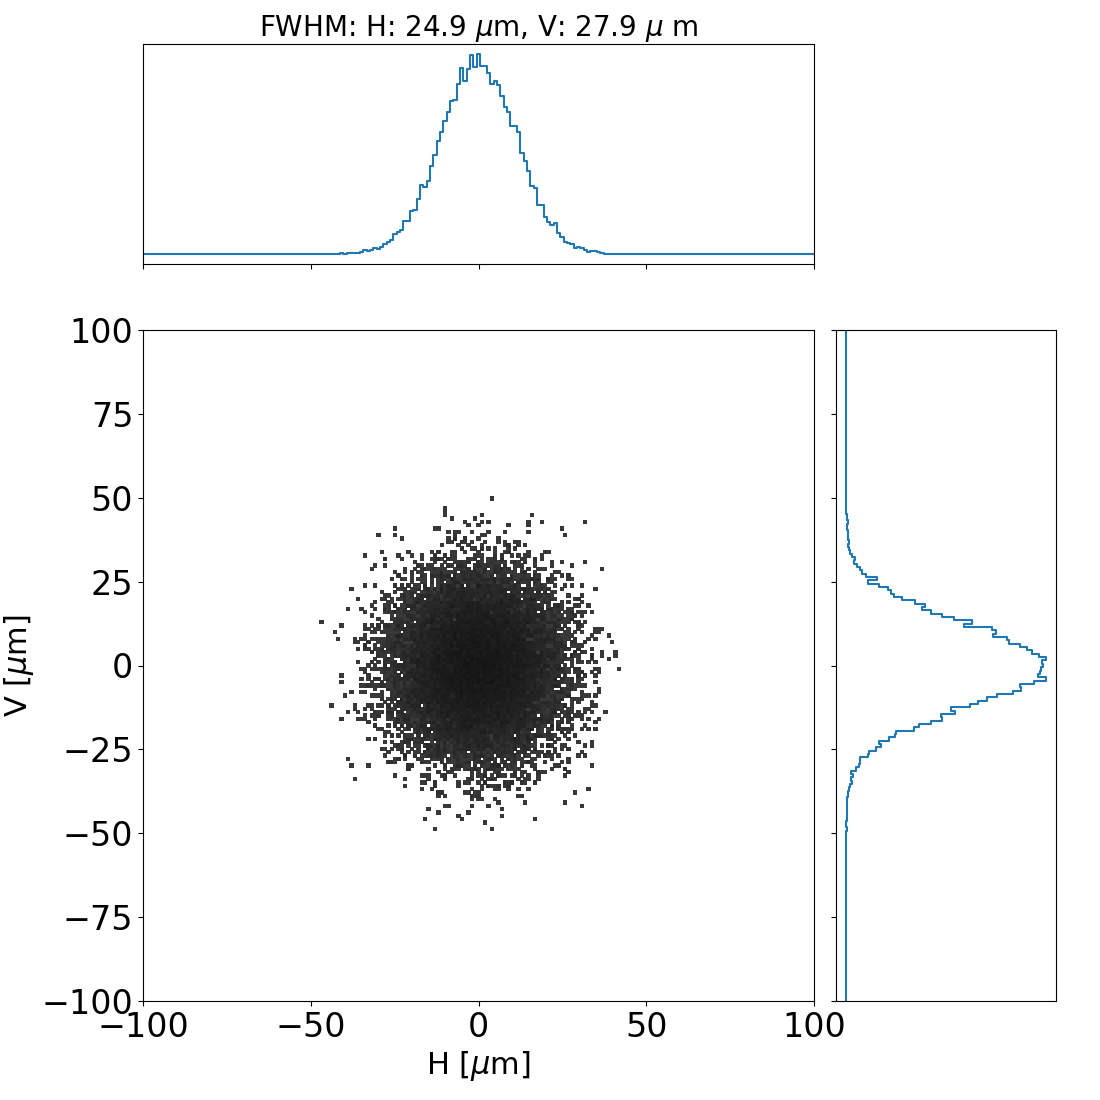
\includegraphics[width=0.45\textwidth]{figures/als_diaboloid.png} \\

\flushleft
~~~~~a$_2$)~~~~~~~~~~~~~~~~~~~~~~~~~~~~~~~~~~~~~~~~~~~~~b$_2$) \\
\centering

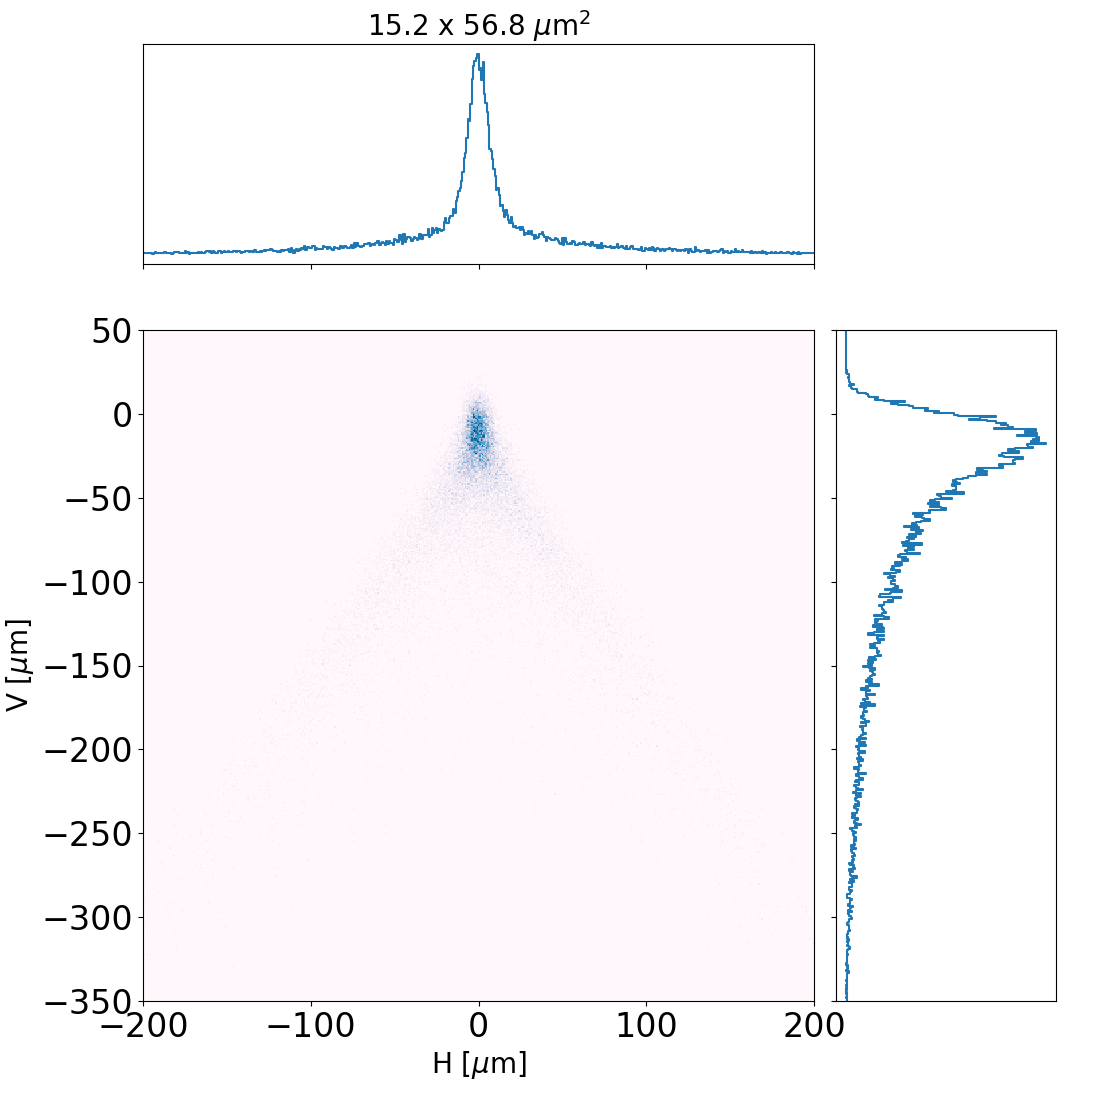
\includegraphics[width=0.45\textwidth]{figures/alsu_toroid.png}
% 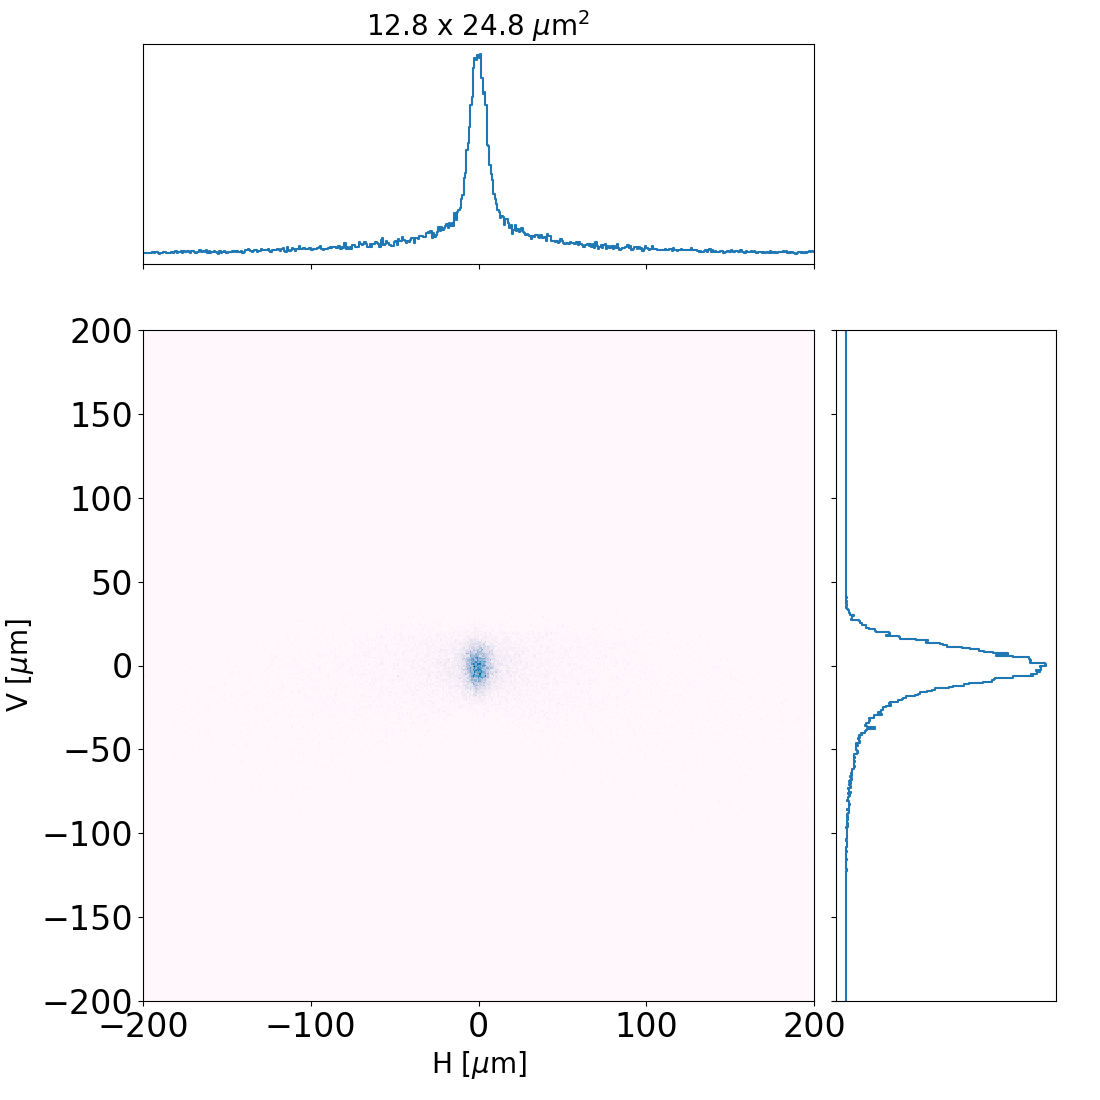
\includegraphics[width=0.32\textwidth]{figures/alsu_parabolic-cone.png}
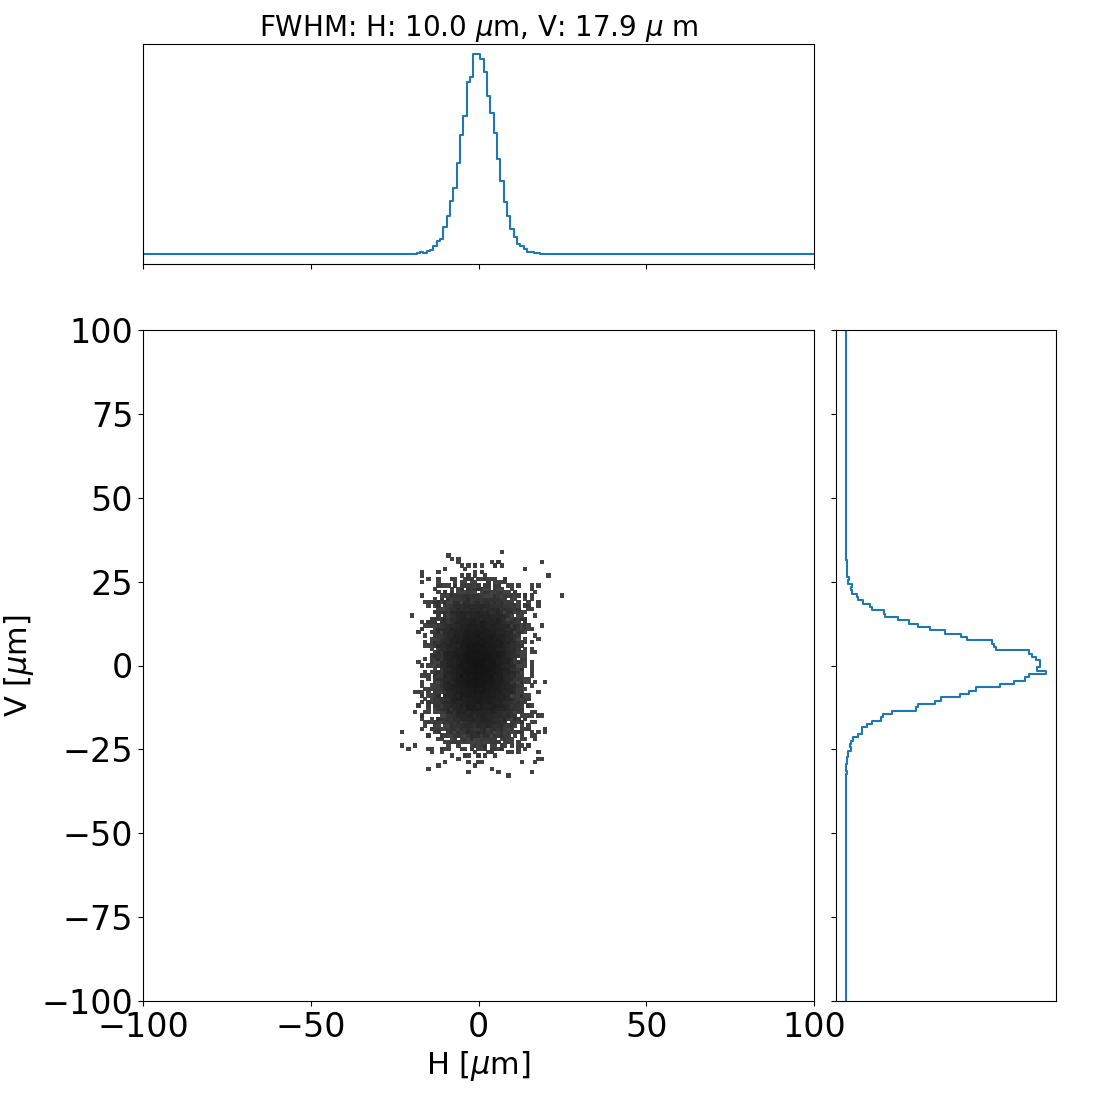
\includegraphics[width=0.45\textwidth]{figures/alsu_diaboloid.png} \\

\flushleft
~~~~~a$_3$)~~~~~~~~~~~~~~~~~~~~~~~~~~~~~~~~~~~~~~~~~~~~~b$_3$) \\
\centering

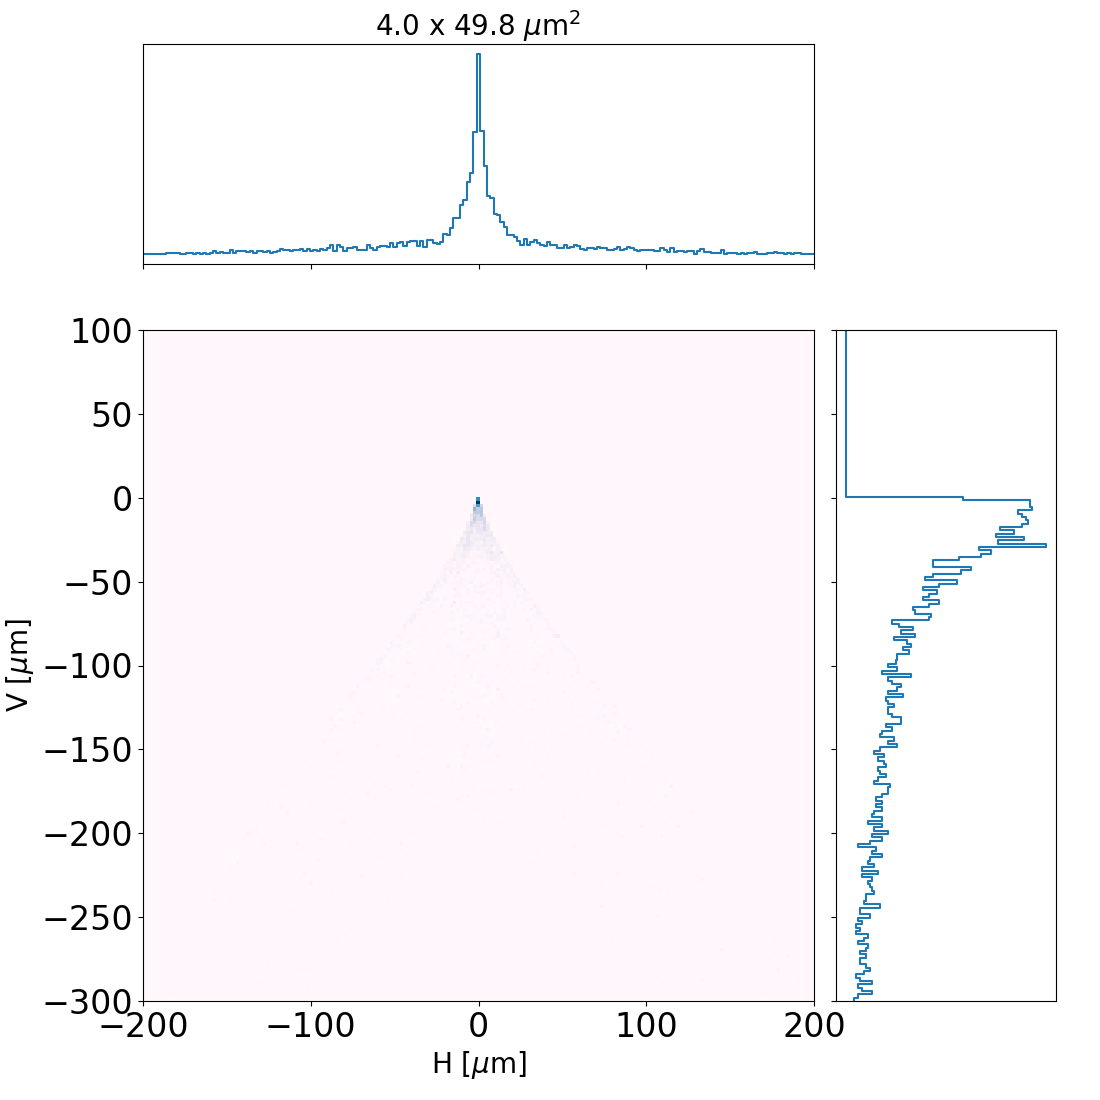
\includegraphics[width=0.45\textwidth]{figures/bl_point_toroid.png} 
% 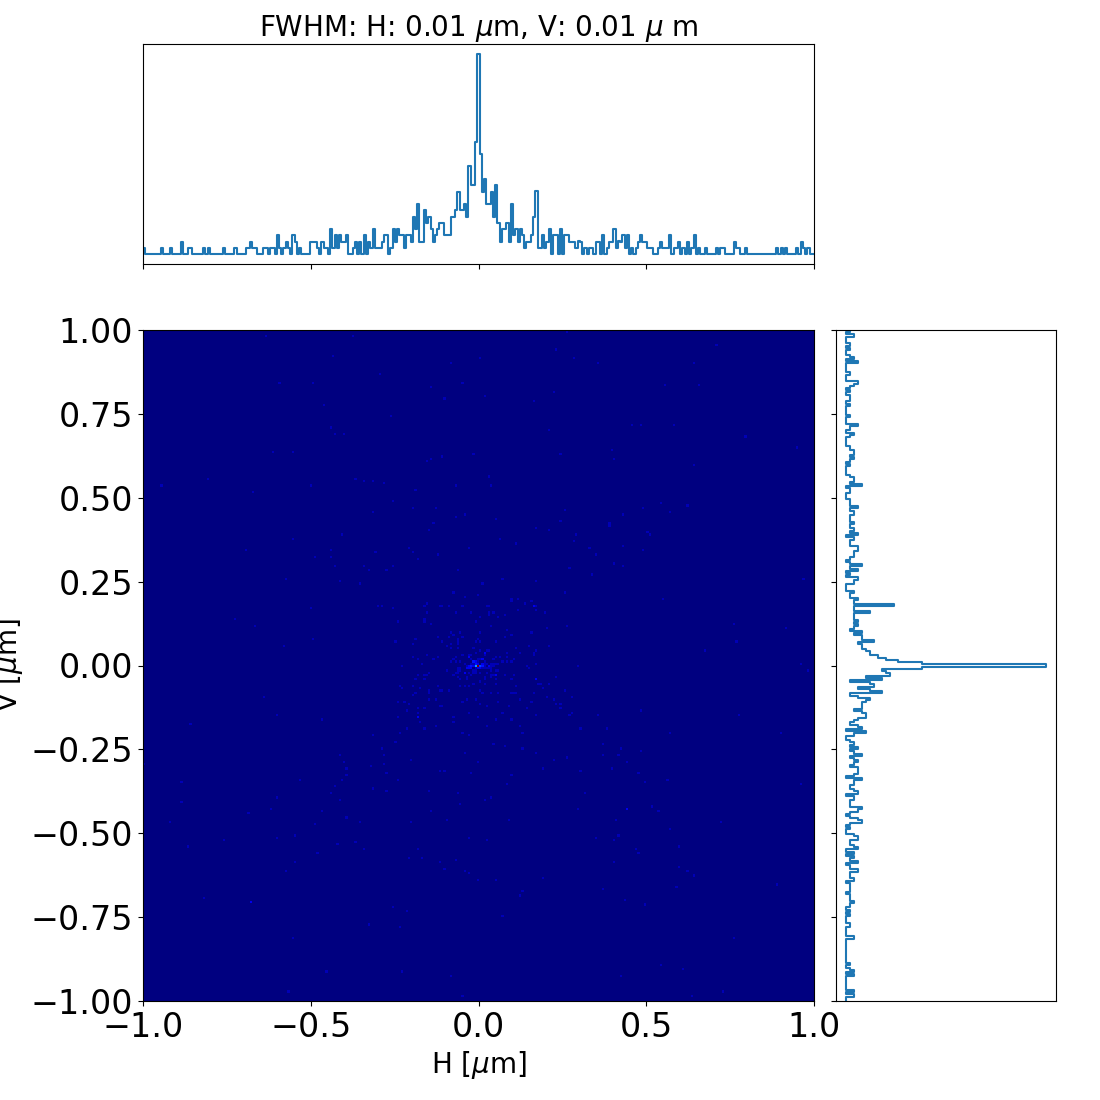
\includegraphics[width=0.45\textwidth]{figures/bl_point_parabolic-cone.png} \\
% \flushleft
% ~~~~~c)~~~~~~~~~~~~~~~~~~~~~~~~~~~~~~~~~~~~~~~~~~~~~d) \\
% 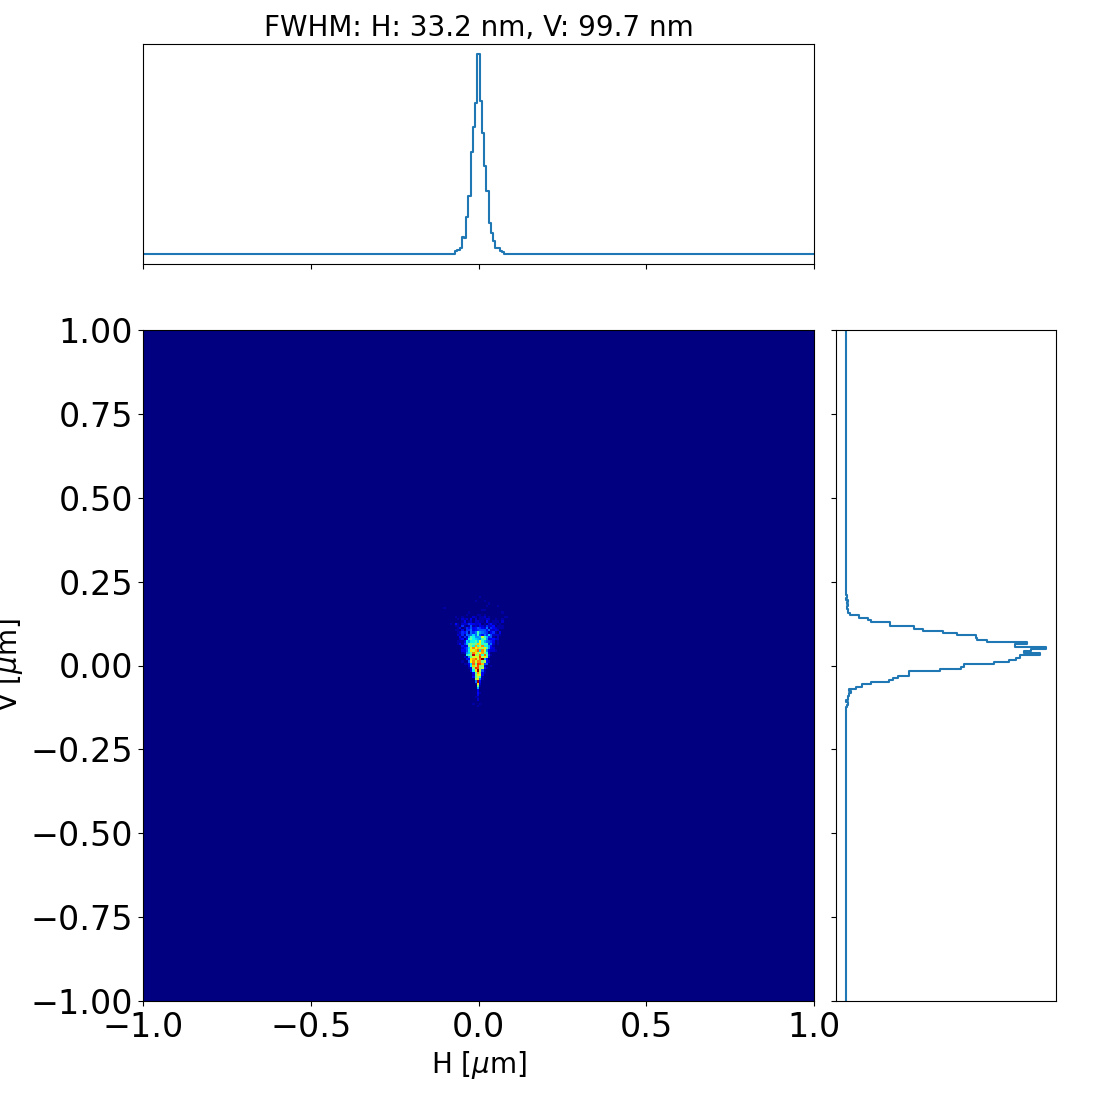
\includegraphics[width=0.45\textwidth]{figures/bl_point_diaboloid.png}
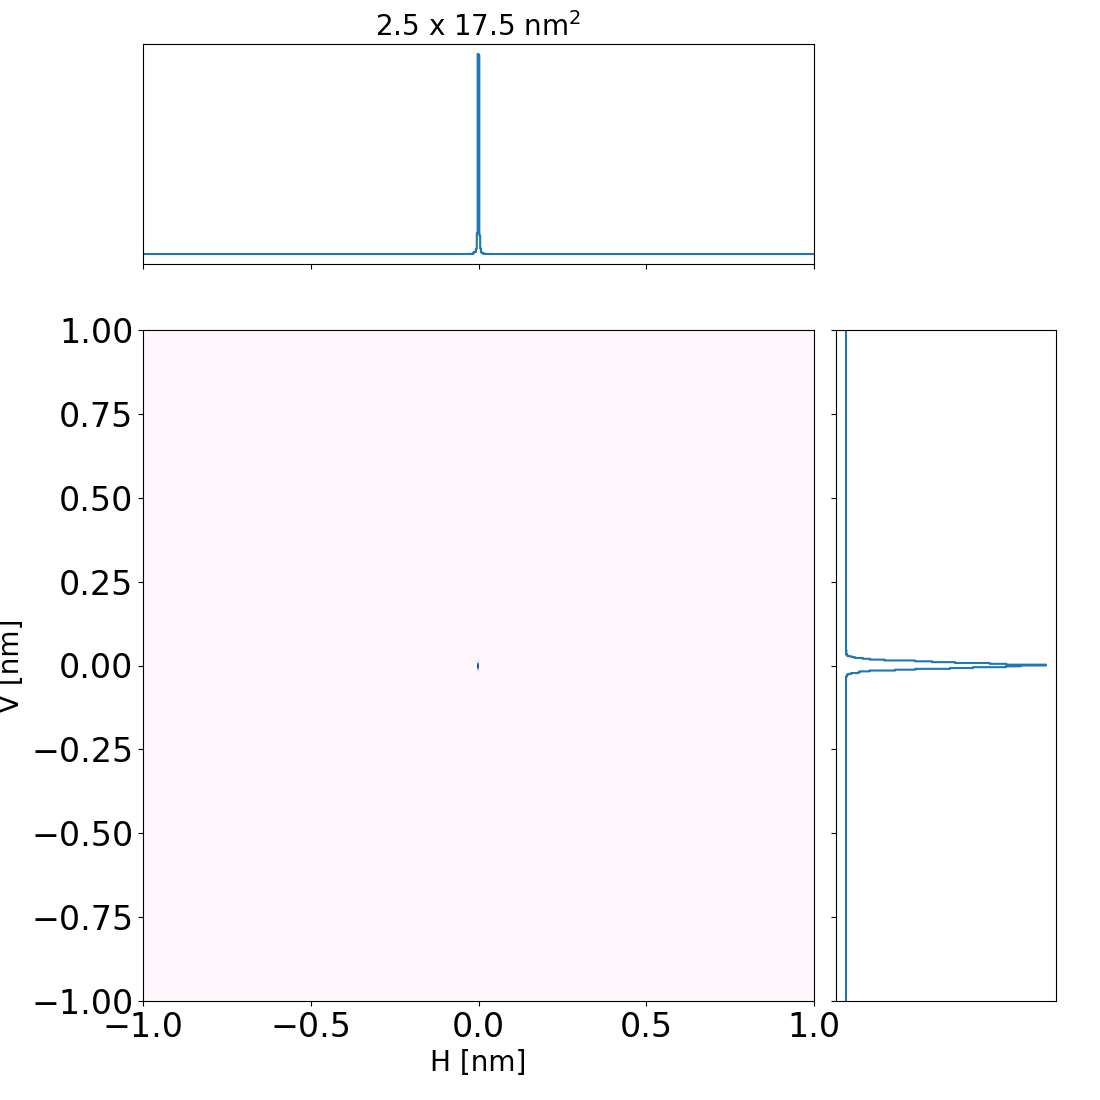
\includegraphics[width=0.45\textwidth]{figures/bl_point_diaboloid-exact.png}  \\
\caption{Focal image produced by a system of two mirrors M1 (collimating parabola) and M2 represented by a a) toroid, b) diaboloid. Row 1 displays the plots for a bending magnet source in the current ALS storage ring. Row 2 is for the upgraded ALS-U ring, and in Row 3 a point source was used. The width values (FWHM) of the intensity distributions are written in the graphic titles. The images contrast is set to logarithmic scale for better visibility. \todo{REMOVE ROW 3?}
}
\end{figure}

In Fig.~\ref{fig:als} we compared the images produced by the beamline for a source using the ALS and ALS-U bending magnets. For the ALS case, the diaboloid obviously improves the toroid case currently impemented, but the gain is not dramatic: a factor 2 in vertical FWHM and less in horizontal, which justifies the use of toroids because manufacturing diaboloids is still a challenge. For the ALS-U the gain of using diabloids is increased to almost a factor 3 in FWHM vertical, which for the toroid is dominated by aberrations.
The use of a point source helps to address the residual widths for the diaboloid, because it should give zero width. As discussed in the previous section, numeric and sampling errors produce here a nanometric-size residual, which is negligeable with respect of the contribution of the source size.

It can be concluded that for the ALS-U there is a significant improvement in the focal image if the toroid is replaced by a diaboloid.
 

\section{The use of diaboloid for high demagnification}
\label{sec:scan}

In this section we study a possible upgrade of the beamline to obtain a smaller spot size. For that the magnification of the beamline has to be reduced. We study the beamline presented in the last section for ALS-U where the exit arm of the M2 mirror is reduced to have a smaller magnification M=$q/p$. The position of M2 is not changed therefore the length of the beamline is not constant. We have performed ray tracing simulations where the M factor is changed to values 1:5 and 1:10 (Fig.~\ref{fig:demagnification}). It can be observed the extremely high aberrations produced by the toroid, which makes its use impossible for these configurations. On the contrary, the diaboloid produces nice Gaussian non-aberrated intensity profiles, as expected.
%Interestingly, the parabolic-cone completely removed all the aberration in the toroid presented in the vertical direction producing very good results of beam size FWHM. However, the intensity in horizontal is closer to the toroid than the diaboloid, with a shape that looks more Lorentzian than Gaussian (higher tails). In vertical the parabolic-cone produces a very clean spot, but not as good as the diaboloid. 


\begin{figure}\label{fig:demagnification}
\flushleft
~~~~~a$_1$)~~~~~~~~~~~~~~~~~~~~~~~~~~~~~~~~~~~~~~~~~~~~~b$_1$) \\
\centering
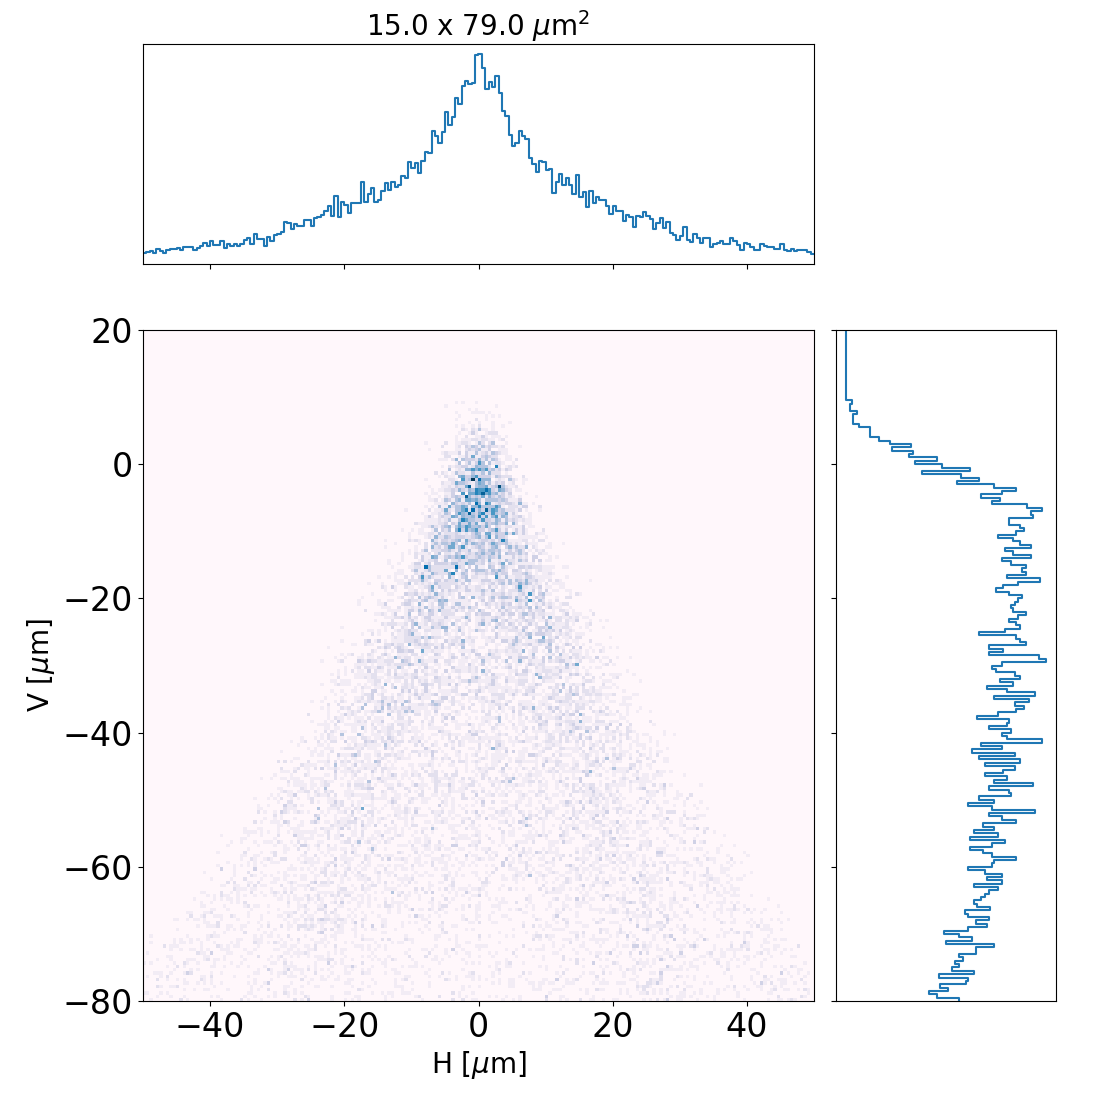
\includegraphics[width=0.45\textwidth]{figures/M0p2_toroid.png}
% 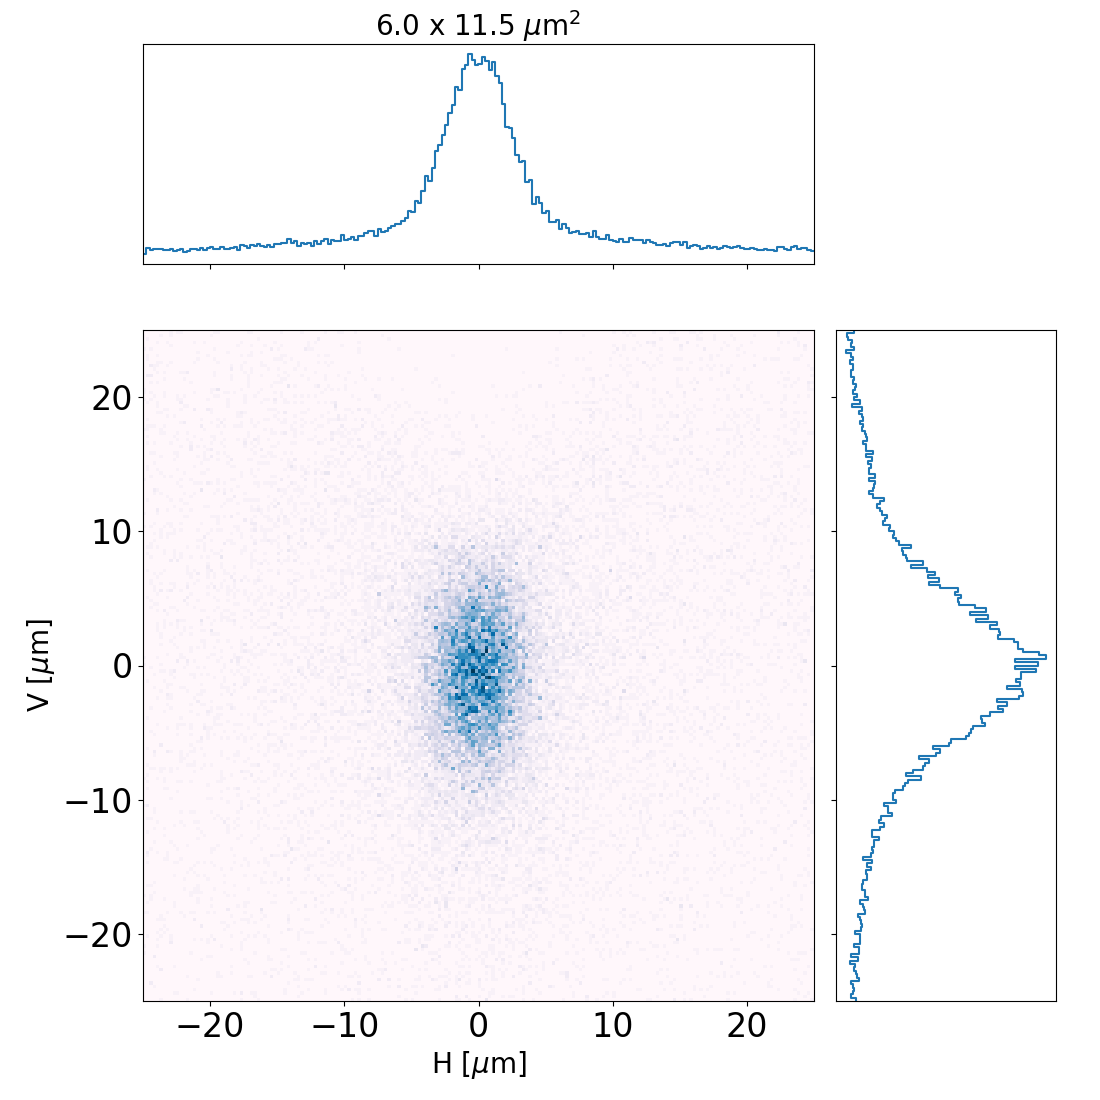
\includegraphics[width=0.32\textwidth]{figures/M0p2_parabolic-cone.png}
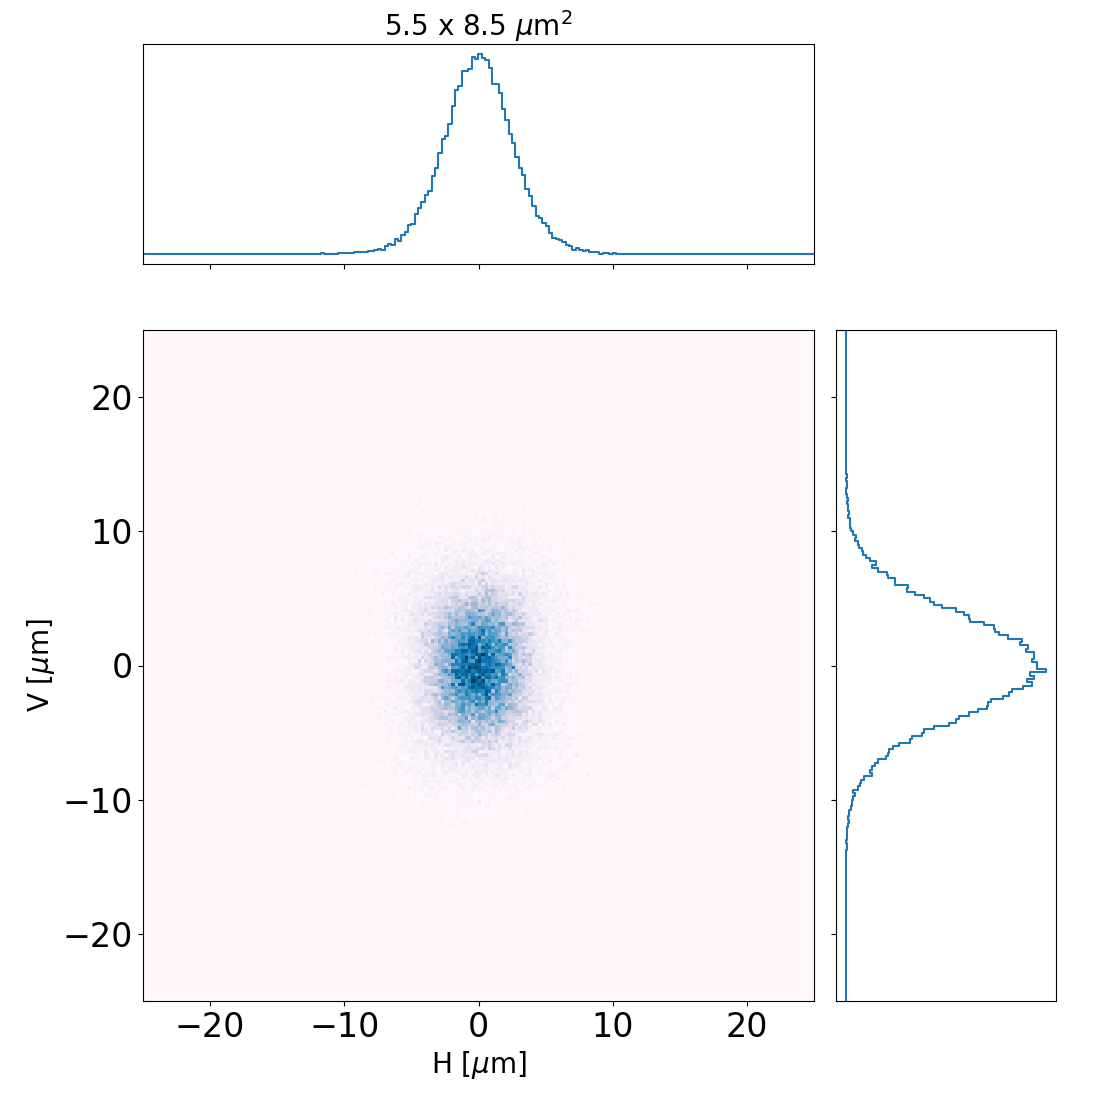
\includegraphics[width=0.45\textwidth]{figures/M0p2_diaboloid.png} \\

\flushleft
~~~~~a$_2$)~~~~~~~~~~~~~~~~~~~~~~~~~~~~~~~~~~~~~~~~~~~~~b$_2$) \\
\centering

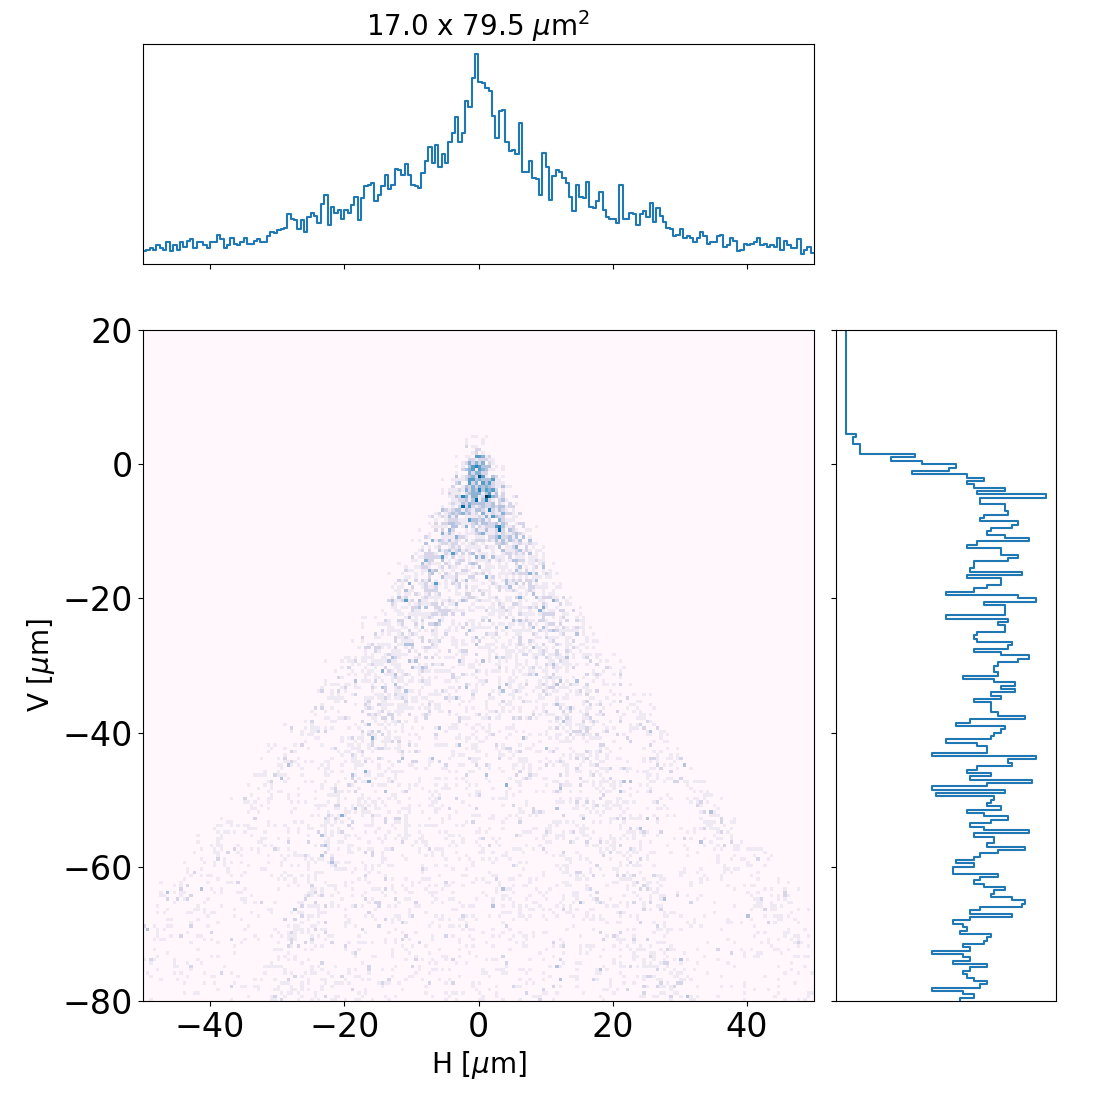
\includegraphics[width=0.45\textwidth]{figures/M0p1_toroid.png}
% 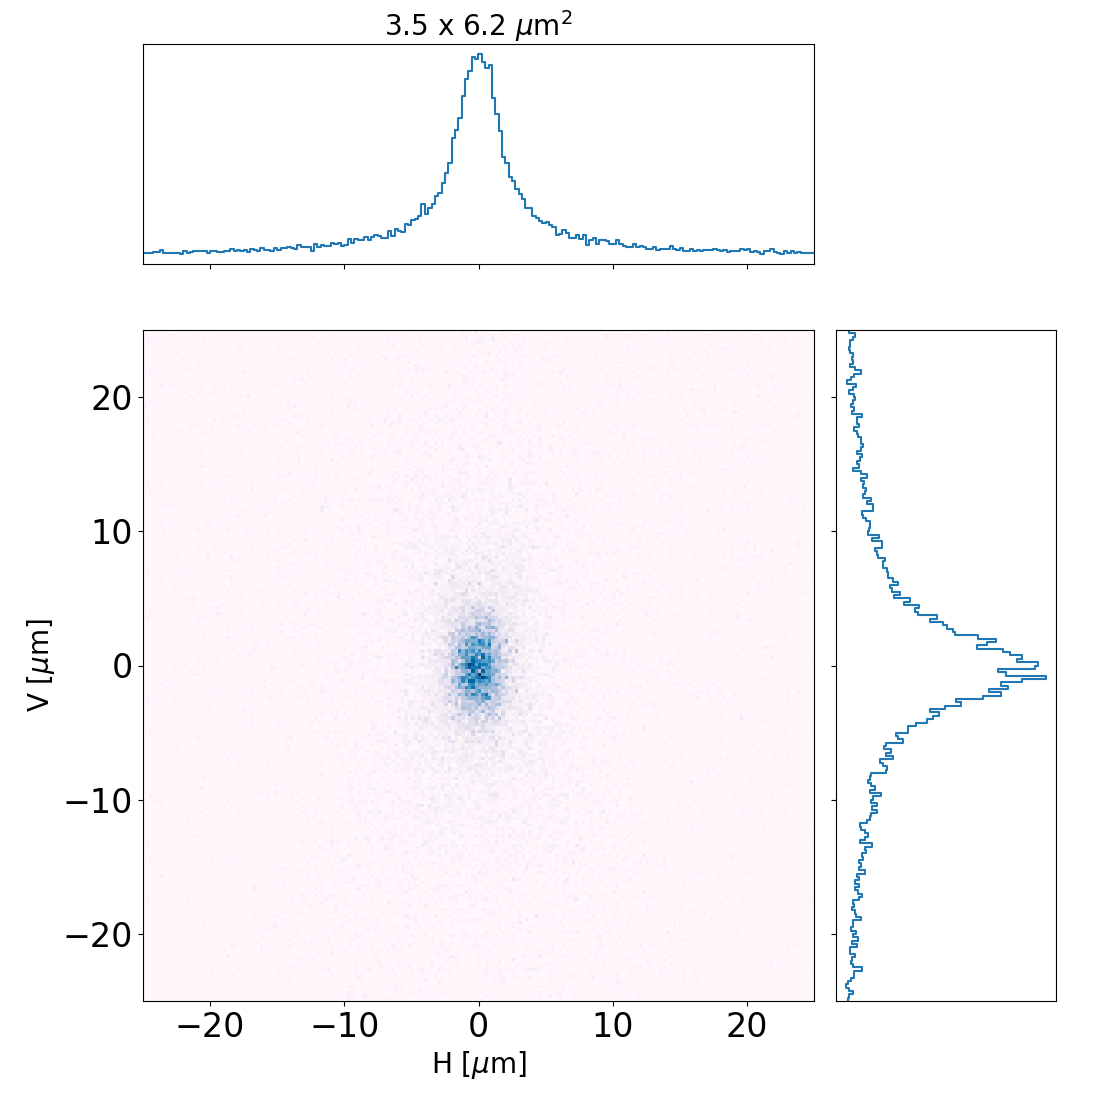
\includegraphics[width=0.32\textwidth]{figures/M0p1_parabolic-cone.png}
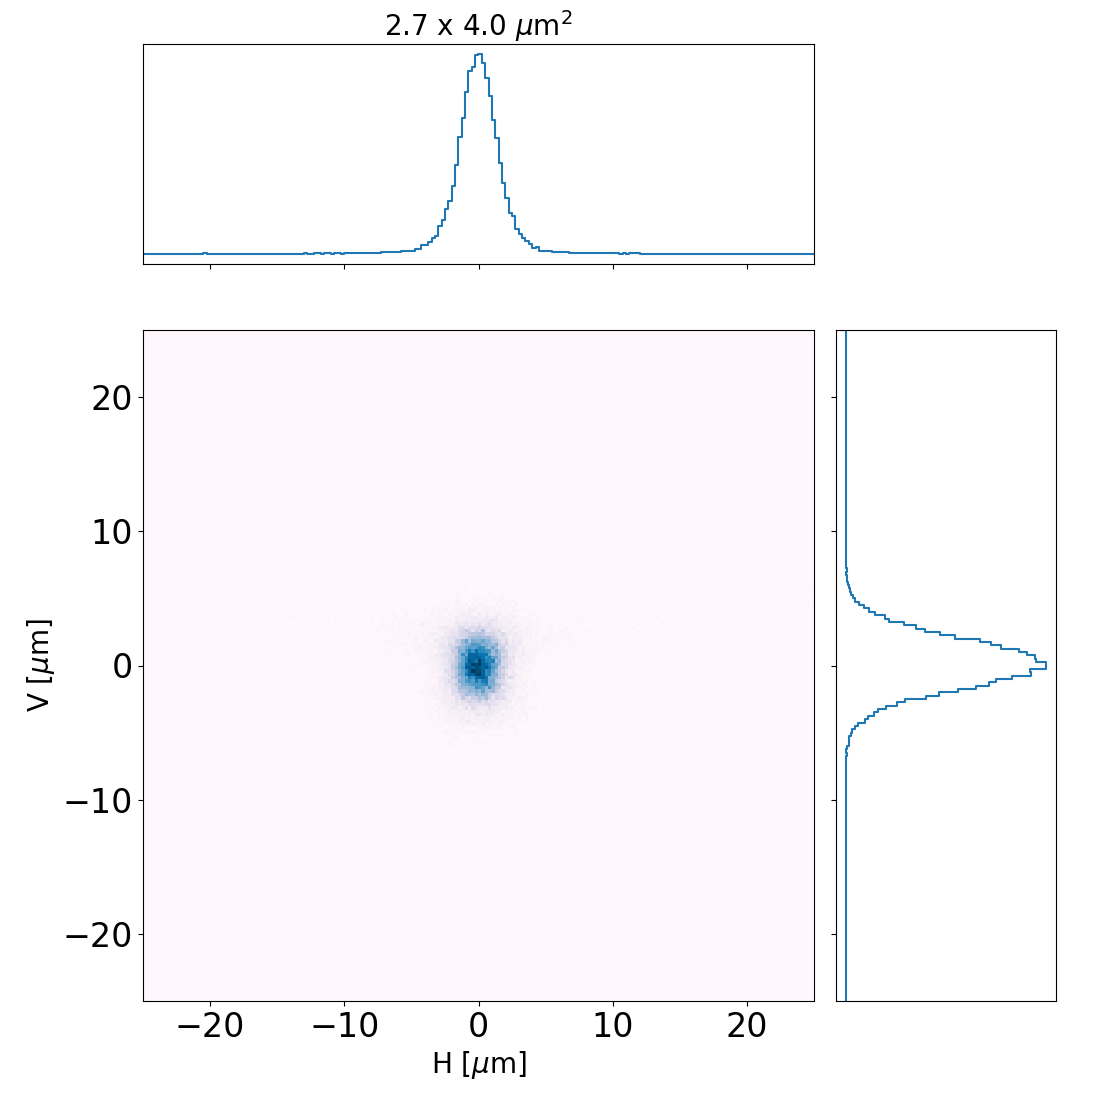
\includegraphics[width=0.45\textwidth]{figures/M0p1_diaboloid.png}
\caption{
Image produced by the beamline for two high demagnification values: 1:5 (row 1, top) and 1:10 (row 2, bottom) using for M2 a) toroid, and b) diaboloid.}
\end{figure}


To study in more detail the aberrations, ray tracing calculations are performed scanning the magnification factor and extracting the focal dimensions. For each ray tracing simulation this focal dimension is calculated in two ways: i) the FWHM of the intensity distribution (as discussed previously), and ii) the standard deviation $\sigma$ of the ray coordinates contributing to the focal image. The purpose is to evaluate the aberrations by comparing the FWHM with $\sigma$. If the intensity distribution is Gaussian, we will obtain a $\sigma$ smaller than the FWHM by a factor 2.35. However, when aberrations are present the long tails make that the $\sigma$ increases rapidly becoming even greater than the FWHM value. If this happens it is an indicator of high aberrations.  

\begin{figure}\label{fig:scan}
\flushleft
a)\\
\centering
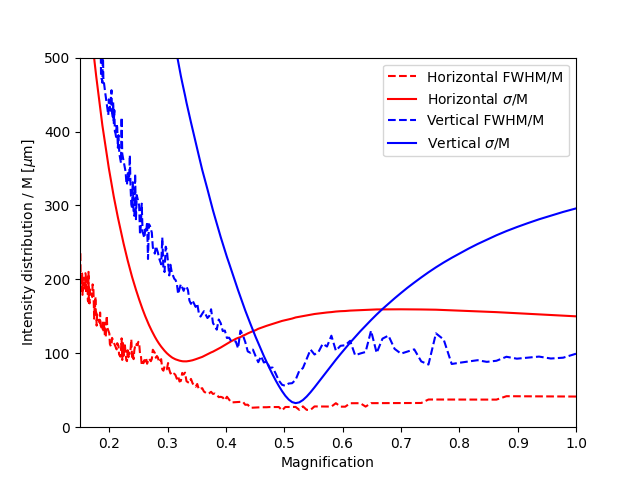
\includegraphics[width=0.95\textwidth]{figures/scan_toroid.png}\\
\flushleft
b)\\
\centering
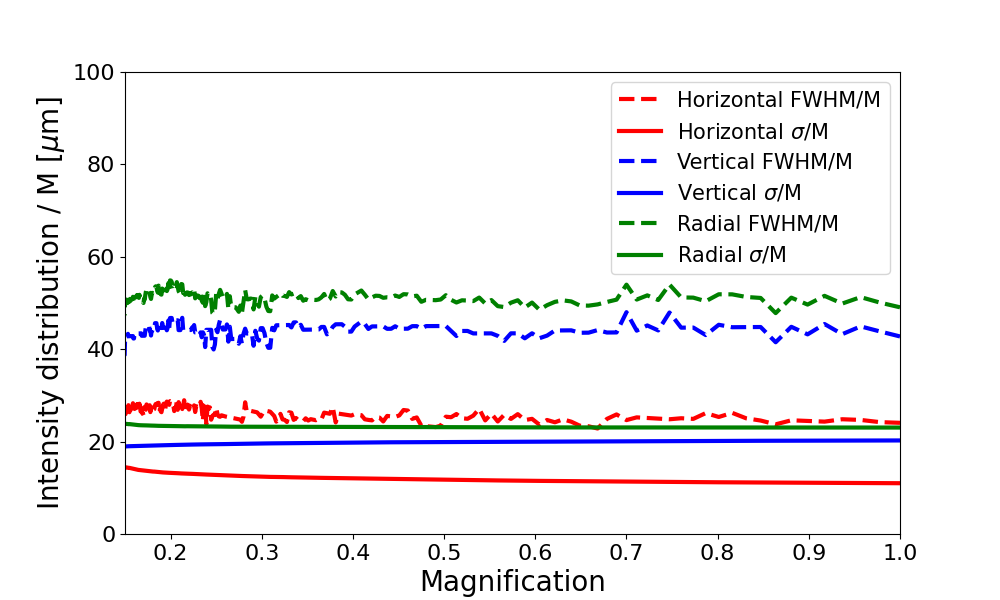
\includegraphics[width=0.95\textwidth]{figures/scan_diaboloid.png}\\
% c)
% 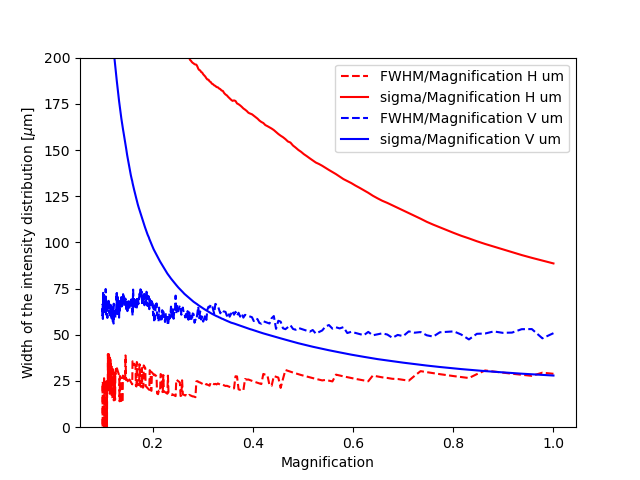
\includegraphics[width=0.95\textwidth]{figures/scan_parabolic-cone.png}

\caption{
Evolution of the (horizontal and vertical) focal size (measured in FWHM and $\sigma$) normalized to the magnification M versus magnification for a beamline with focusing M2 mirror shape: a) toroid, and b) diaboloid. The normalized focal size should be a constant for a perfect optics.
}
\end{figure}


Fig.~\ref{fig:scan} shows the results of ray tracing calculations of the focal size versus magnification M. Because the size is proportional to the magnification (in the ideal case of zero aberrations), we have visualized the focal size (in FWHM or $\sigma$ for horizontal and vertical directions) divided by the magnification in order to obtain an constant value in the ideal case of zero aberrations. Looking at the response of the toroidal mirror we can identify large aberrations for most cases (the $\sigma$ values are higher than the FWHM) and there is an optimum value around M=0.5 where the vertical size is minimum. This is the "working condition" of most beamlines using toroids at ALS as the aberrations are minimized \cite{MacDowell2004}. For the diaboloid (Fig~\ref{fig:scan}b) the situation is completely different. For most of cases (M$>$0.2) the lines are almost constant and the $\sigma$'s smaller than the FWHM by a value approaching 2.35, indicating that the diaboloid behaves as a perfect optics. 
%For the parabolic-cone (Fig~\ref{fig:scan}c) the situation is very close to the diaboloid when looking at the FWHM values down to the minimum M. When the values of $\sigma$ are higher than FWHM there is presence of residual aberrations. This is true for the horizontal focus, an effect already observed in the previous section, and it is less important for the vertical direction: only for M$<$0.3 the $\sigma$ becomes higher that the FWHM.  




\section{Study of mirror shapes that approximate the diaboloid}
\label{sec:approximatedShapes}

The diaboloid is a highly aspherical surface in both directions, with sagittal section an ellipse and tangential section a parabola. The fabrication of such a surface within the required accuracy required for practical application in an X-ray beamline is a challenging technological problem. 




%A realisable approximation of the diaboloid surface could be made by dynamical mechanical bending of a substrate pre-shaped to the sagittal curvature. The dynamical bending would form the tangential shape onto the tangentially flat substrate. This approach is used in many existing toroidal mirrors, where the toroid is obtained by dynamically curving to a circular (tangential) shape a pre-shaped (sagittal) cylinder. By replacing the pre-shape cylinder by a aspheric section, and then apply adequated bending moments one could perhaps approximate well the diaboloid and benefit its superior performances in a beamline. Two solutions may be envisaged for the pre-shaped cone. The first one is to approximate the elliptical sagittal profile to a circular profile that linearly changes along the $Y$ (tangential) direction following the Eq.~\ref{eq:sagRadius}. A second one, more precise at a first view, would consist in pre-shaping a cone with elliptical (sagittal) section. However, these ellipses are different for different $Y$. 

%This cone degenerates in a cylinder for 2:1 demagnification. Again, this variation is null for 2:1 demagnification becoming a cylinder with elliptical section, which could be envisaged to be manufactured. 

To assess the feasibility of manufacturing a diaboloid-like surface it is convenient to analyze the height differences between the diaboloid and the toroidal surface which is spherical in both directions. With the Oasys Diaboloid widget we can easily substract the best toroid from the diaboloid. In Fig.~\ref{fig:detrended}a we have analysed diaboloid surfaces for different magnification (1:5, 1:2 and 1:1) and grazing angles 2 mrad. For all surfaces $p$=20 m and the best toroid has been removed, in order to study the aspherical components. Some sagittal profiles are also shown. It can be appreciated in the magnification 1:5 ($p$=20 m, $q$=4m) and 1:1 ($p$=$q$=20) a slight variation of the sagittal profile when going from one edge ($Y$=-100 mm) to another ($Y$=100 mm). However the change of height is abour 100 $\mu$m for the first and 6 $\mu$m for the second. 

%As expected (discussed in \cite{part2} Section 6), for 1:2 magnification the sagittal profiles are almost identical as a result of vanishing the linear term in Eq.~\ref{eq:sagittalRadiusLinearized}. This case corresponds to the well-known 2:1 demagnification "golden rule" implemented in the crystallography beamlines at the Advanced Light Source. These are good candidate to construct a first approximation to the diabloid. 

At the magic 2:1 demagnification condition, for a 2 mrad grazing angle (Fig.~\ref{fig:detrended}a), the difference from the toroidal shape is at its maximum 25 microns, and for a 5 mrad grazing angle (Fig.~\ref{fig:detrended}b), the difference is 1.4 microns.  The change in height is almost constant in the 2:1 case.  Therefore at least in the 5 mrad case, to convert the cylinder to an ellipse in moving from the toroid to the diaboloid in the sagittal direction, could be done with the addition of a varied thickness coating.  The addition of a few microns of sputtered Si on the Si substrate certainly is practical.  In addition, the unbent mirror at the 2:1 condition is essentially a very long elliptical cylinder.  This should allow convenient ways to check the mirror height error using optical interferometery.  Moreover, experience with long cylinders has shown that they can be produced with surprisingly low tangential slope errors, commensurate with the applications we envision.  The addition of a thin correcting layer at the edge of the cylindrical substrate seems to be an attractive way to make diaboloids at least for the 5 mrad grazing angle case. 










\begin{figure}\label{fig:detrended}
\flushleft
a$_1$)~~~~~~~~~~~~~~~~~~~~~~~~~~~~~~~~~b$_1$)~~~~~~~~~~~~~~~~~~~~~~~~~~~~~~c$_1$)\\
\centering
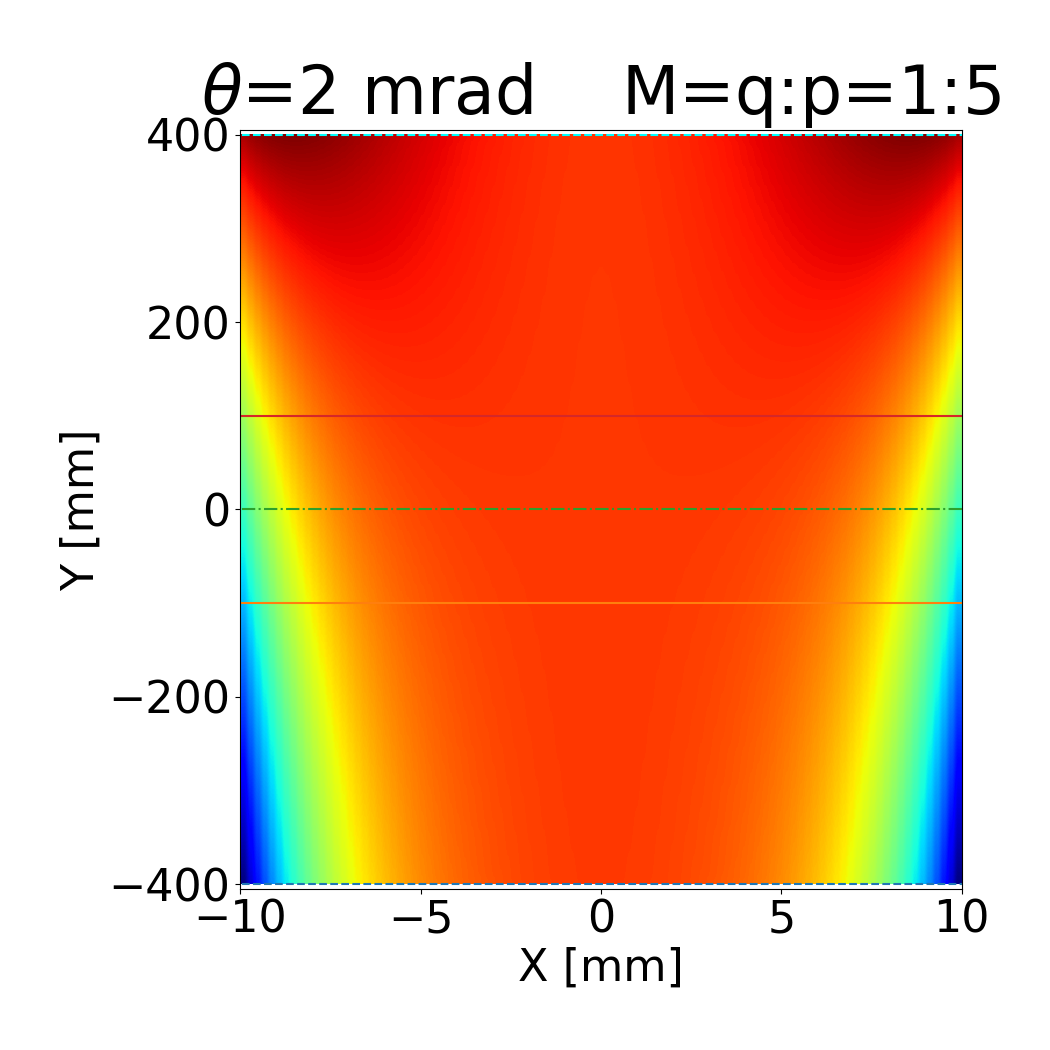
\includegraphics[width=0.32\textwidth]{figures/diaboloid_detrended_1:5_image.png} 
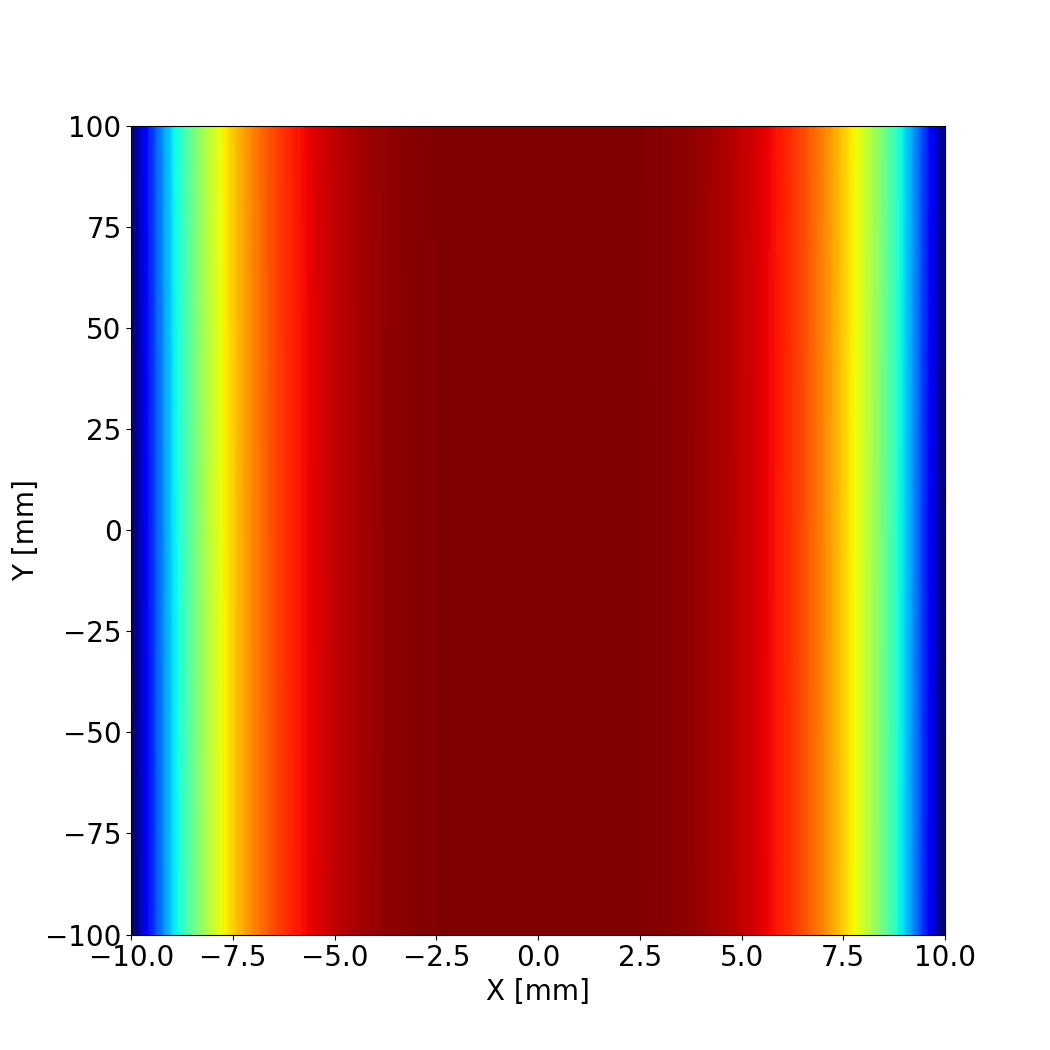
\includegraphics[width=0.32\textwidth]{figures/diaboloid_detrended_1:2_image.png} 
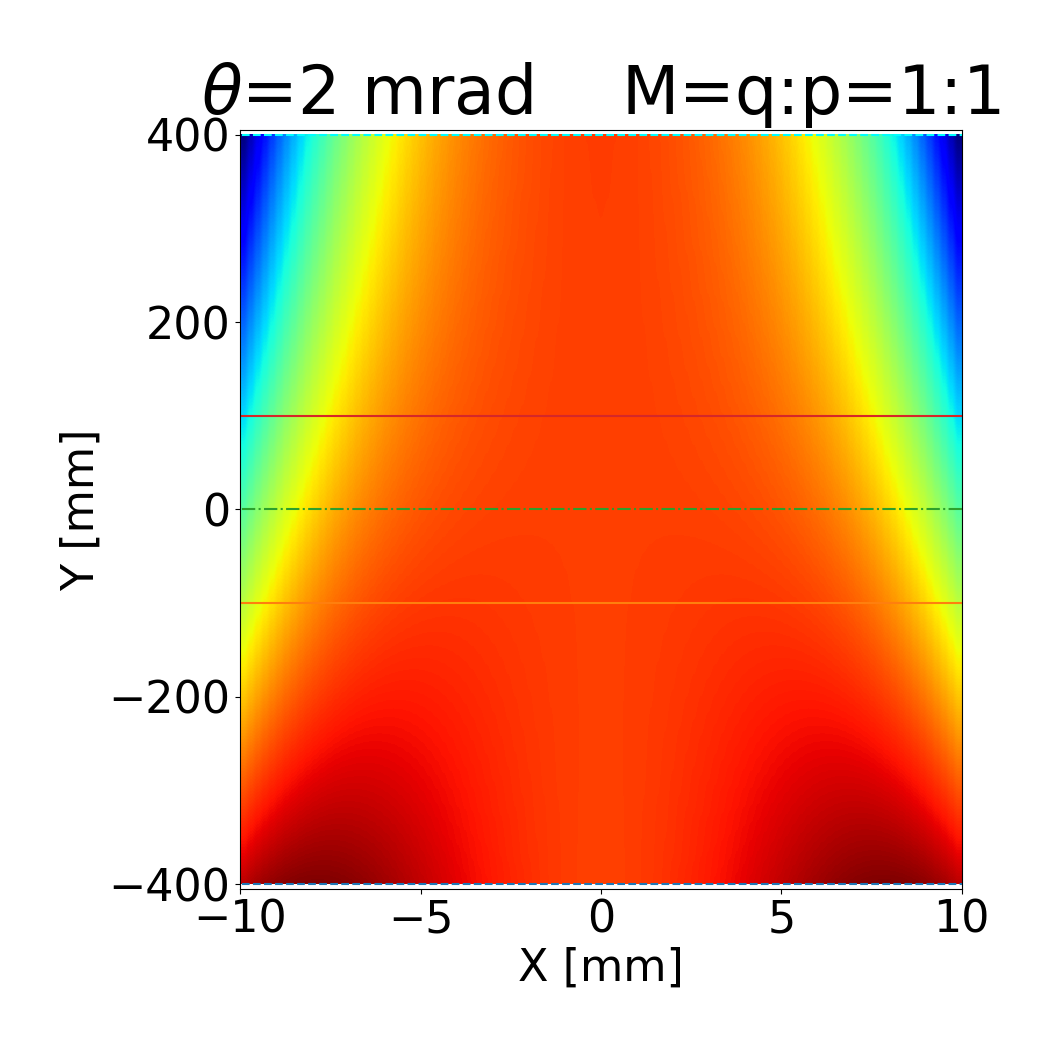
\includegraphics[width=0.32\textwidth]{figures/diaboloid_detrended_1:1_image.png} \\
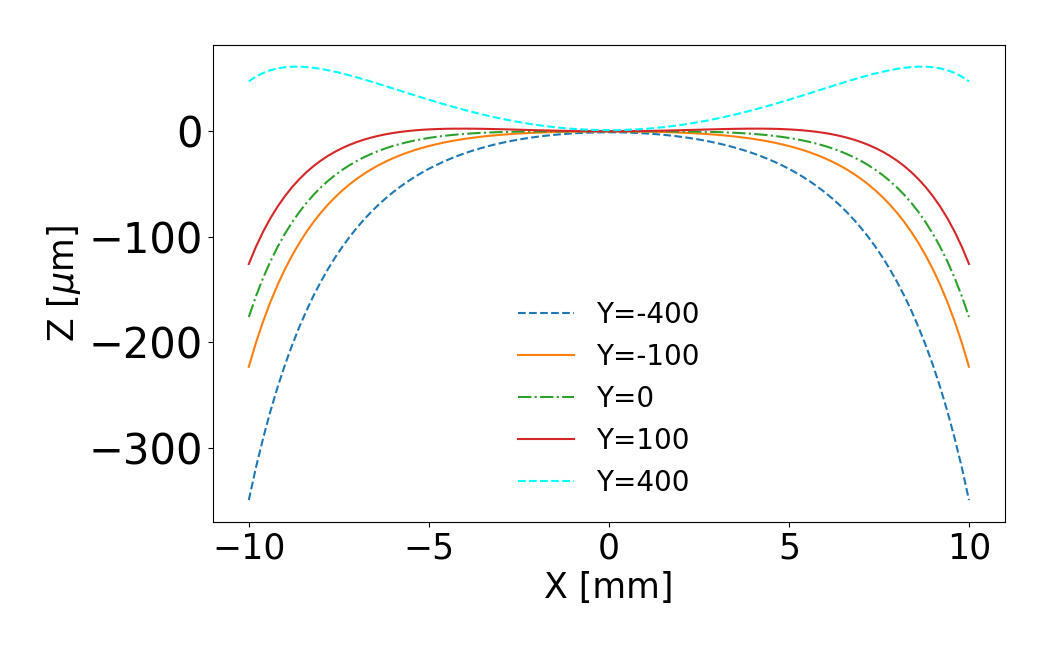
\includegraphics[width=0.32\textwidth]{figures/diaboloid_detrended_1:5_profile.png}
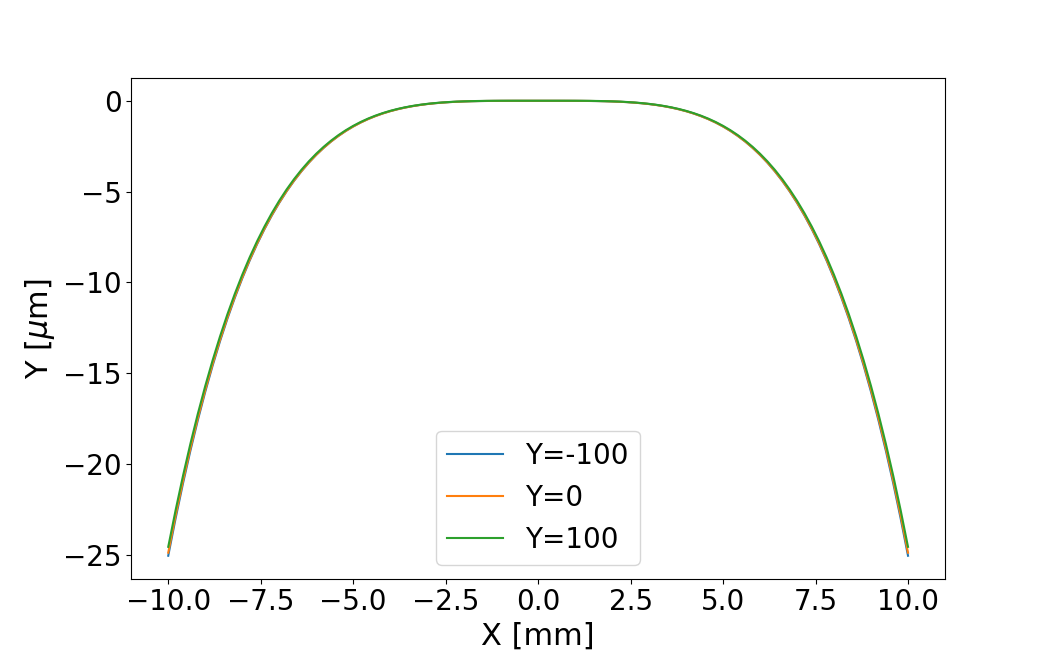
\includegraphics[width=0.32\textwidth]{figures/diaboloid_detrended_1:2_profile.png}
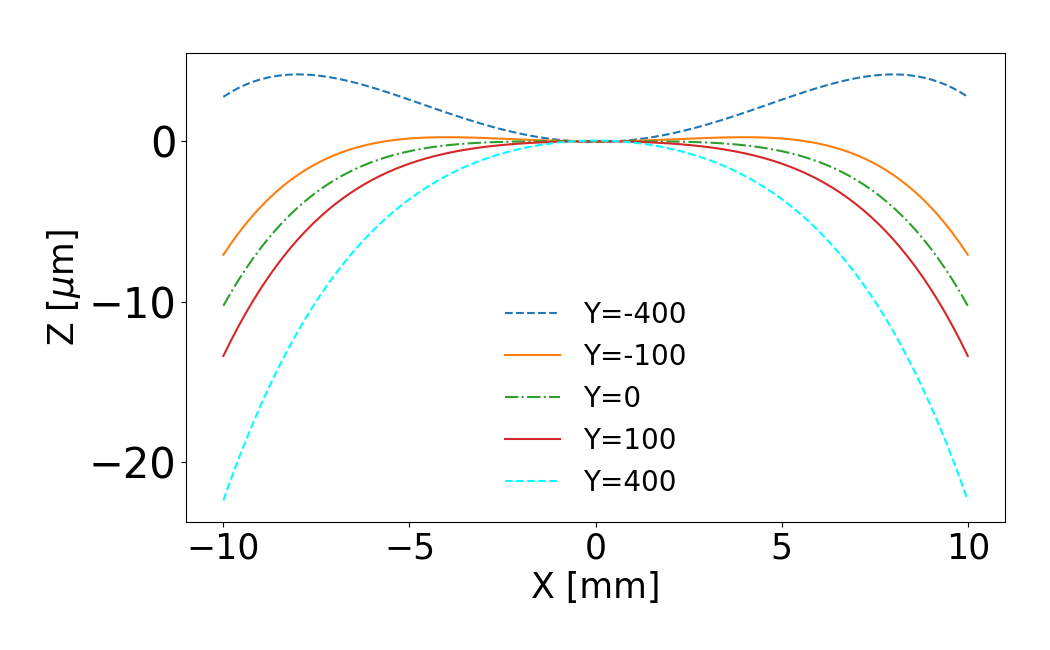
\includegraphics[width=0.32\textwidth]{figures/diaboloid_detrended_1:1_profile.png} \\
\flushleft
a$_2$)~~~~~~~~~~~~~~~~~~~~~~~~~~~~~~~~~b$_2$)~~~~~~~~~~~~~~~~~~~~~~~~~~~~~~c$_2$)\\
\centering
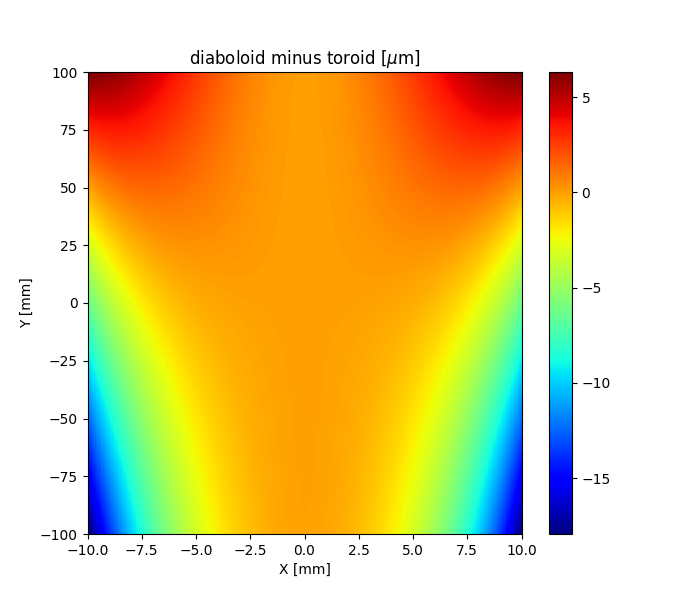
\includegraphics[width=0.32\textwidth]{figures/diaboloid_detrended_5mrad_1:5_image.png} 
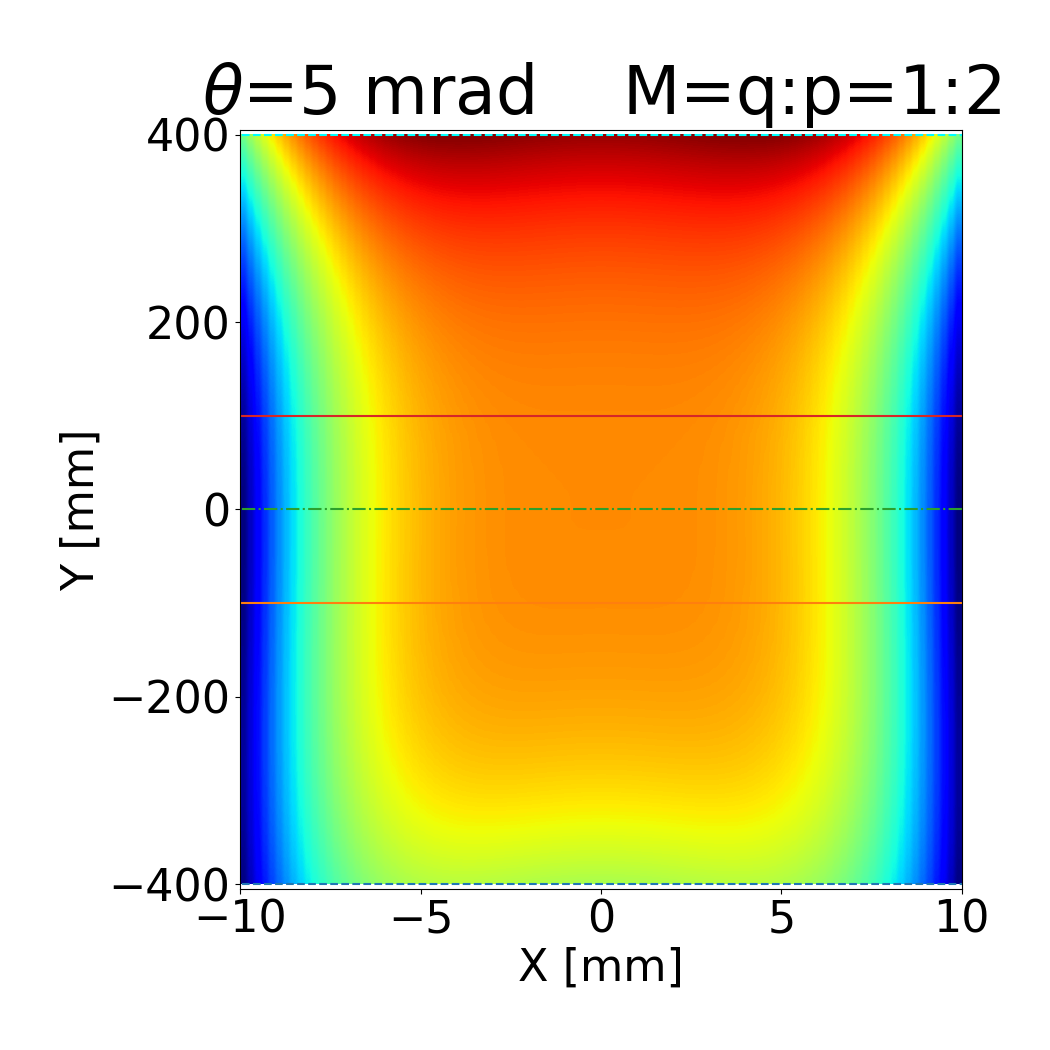
\includegraphics[width=0.32\textwidth]{figures/diaboloid_detrended_5mrad_1:2_image.png} 
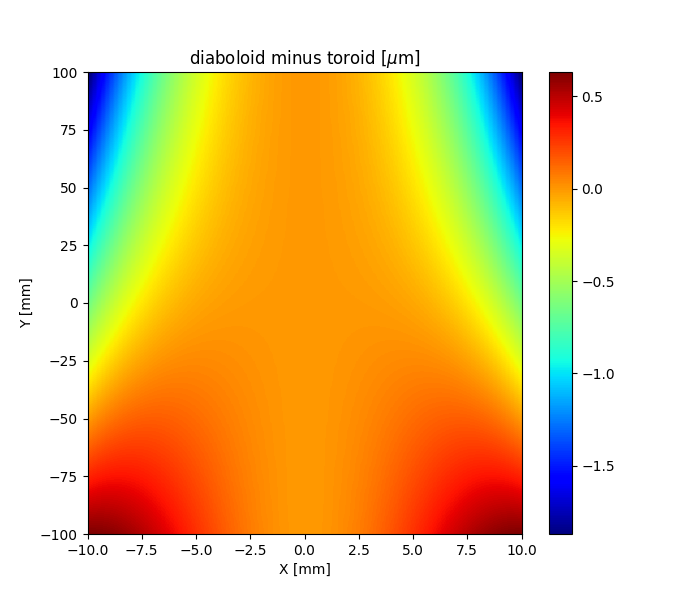
\includegraphics[width=0.32\textwidth]{figures/diaboloid_detrended_5mrad_1:1_image.png} \\
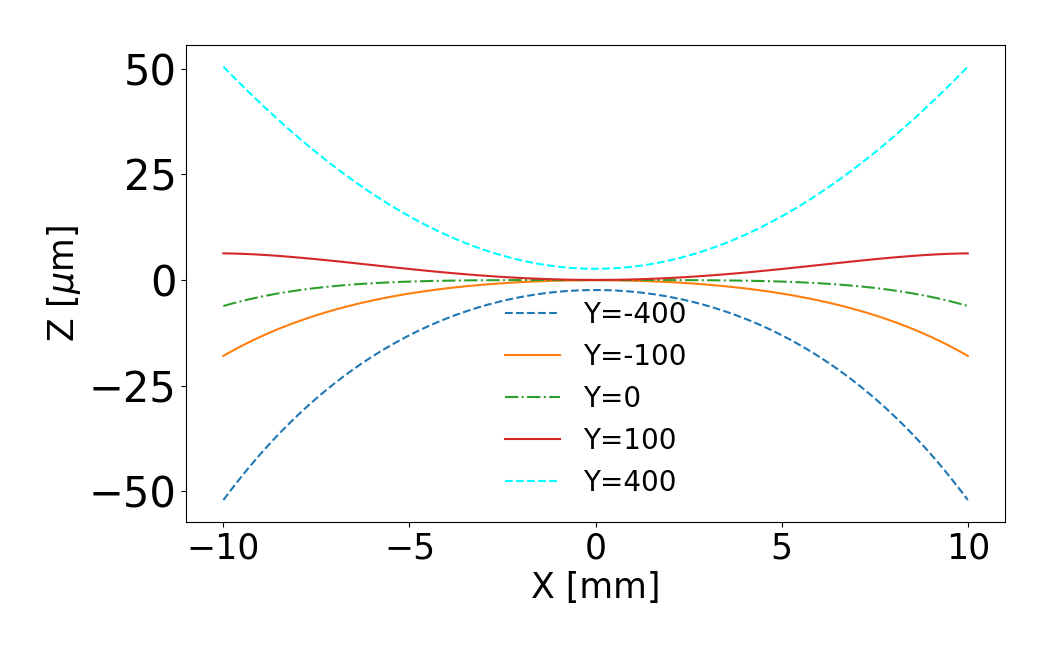
\includegraphics[width=0.32\textwidth]{figures/diaboloid_detrended_5mrad_1:5_profile.png}
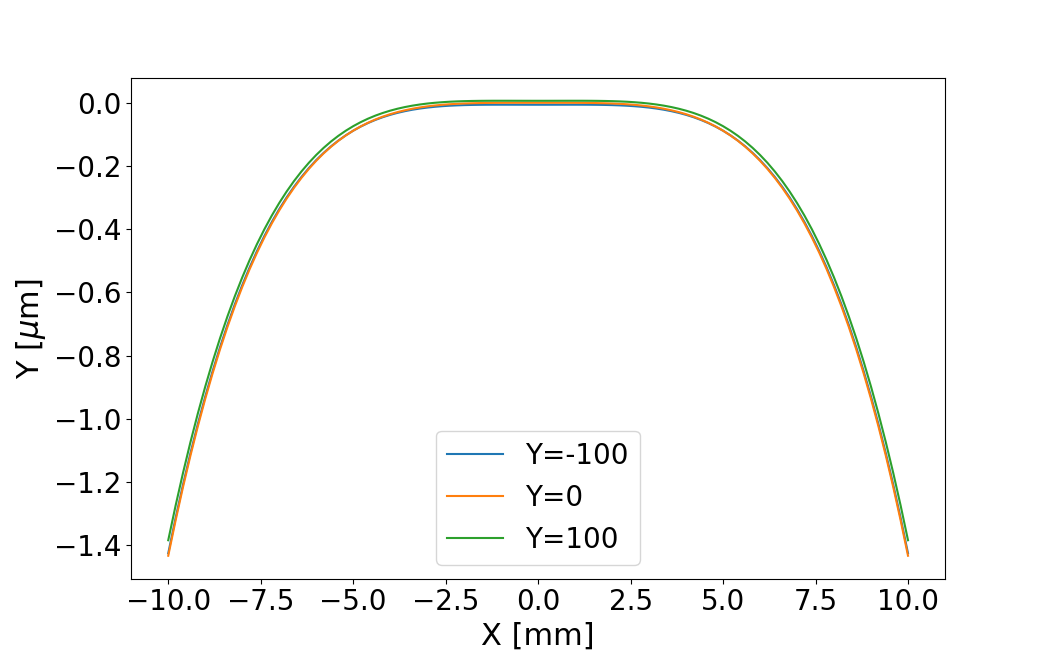
\includegraphics[width=0.32\textwidth]{figures/diaboloid_detrended_5mrad_1:2_profile.png}
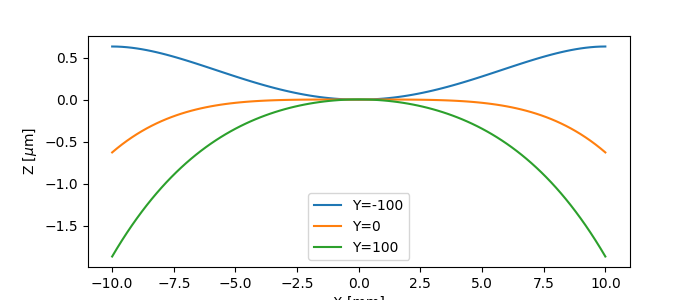
\includegraphics[width=0.32\textwidth]{figures/diaboloid_detrended_5mrad_1:1_profile.png}

\caption{
Height difference between the diaboloid and the toroid for different magnifications a) 1:5, b) 1:2, c) 1:1. In the simulations $p$=20 m and grazing angle is 2 mrad (row 1) or 5 mrad (row 2). The detrended toroid major radii are R$_{a)}$=4 Km, R$_{b)}$=10 Km, R$_{c)}$=20 Km and minor radii r$_{a)}$=13.3 mm, r$_{b)}$=26.7 mm, r$_{c)}$=40 mm for row 1 and R$_{a)}$=1.6 Km, R$_{b)}$=4 Km, R$_{c)}$=8 Km and minor radii r$_{a)}$=33.3 mm, r$_{b)}$=66.6 mm, r$_{c)}$=100 mm for row 2.
}
\end{figure}

% \begin{figure}\label{fig:detrended5mrad}
% \flushleft
% a)~~~~~~~~~~~~~~~~~~~~~~~~~~~~~~~~~b)~~~~~~~~~~~~~~~~~~~~~~~~~~~~~~c)\\
% \centering
% 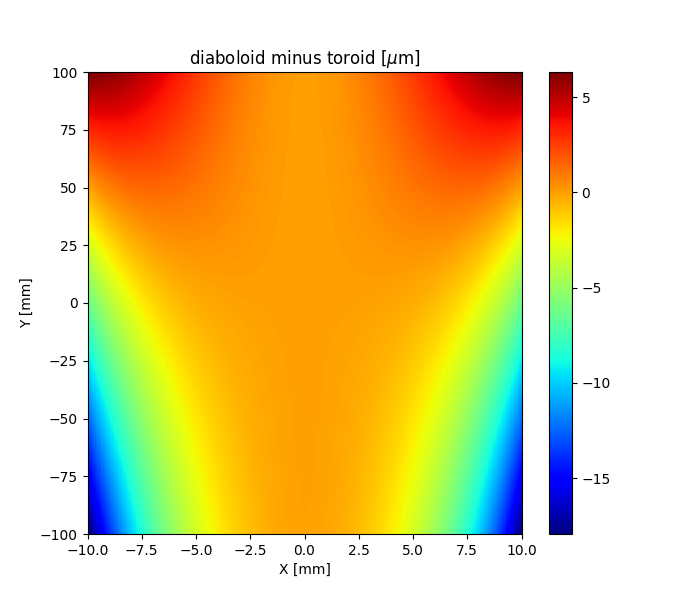
\includegraphics[width=0.32\textwidth]{figures/diaboloid_detrended_5mrad_1:5_image.png} 
% 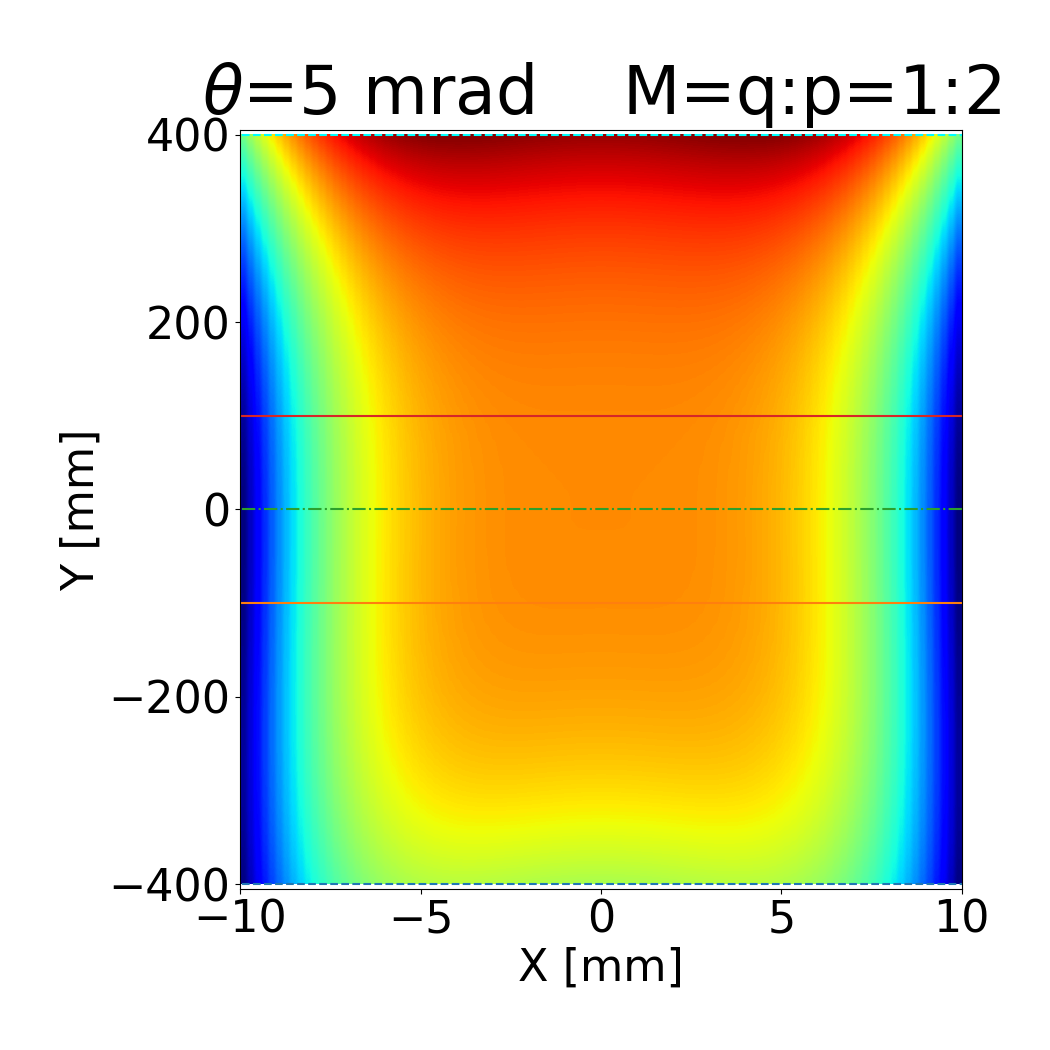
\includegraphics[width=0.32\textwidth]{figures/diaboloid_detrended_5mrad_1:2_image.png} 
% 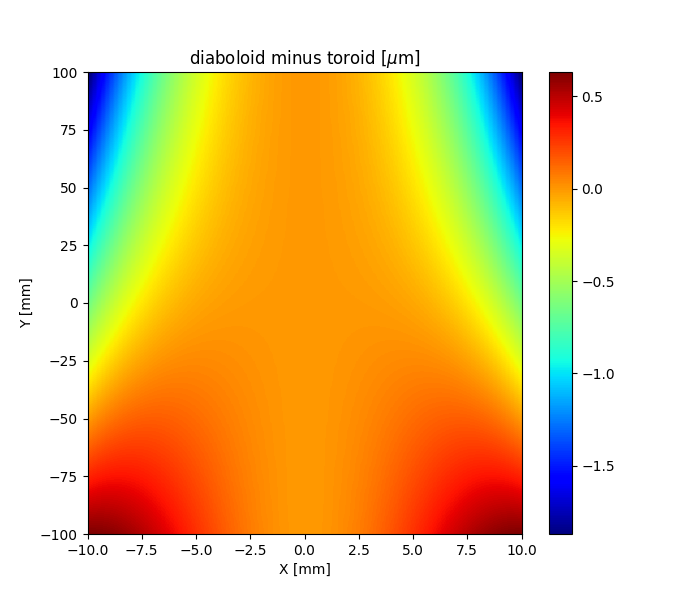
\includegraphics[width=0.32\textwidth]{figures/diaboloid_detrended_5mrad_1:1_image.png} \\
% 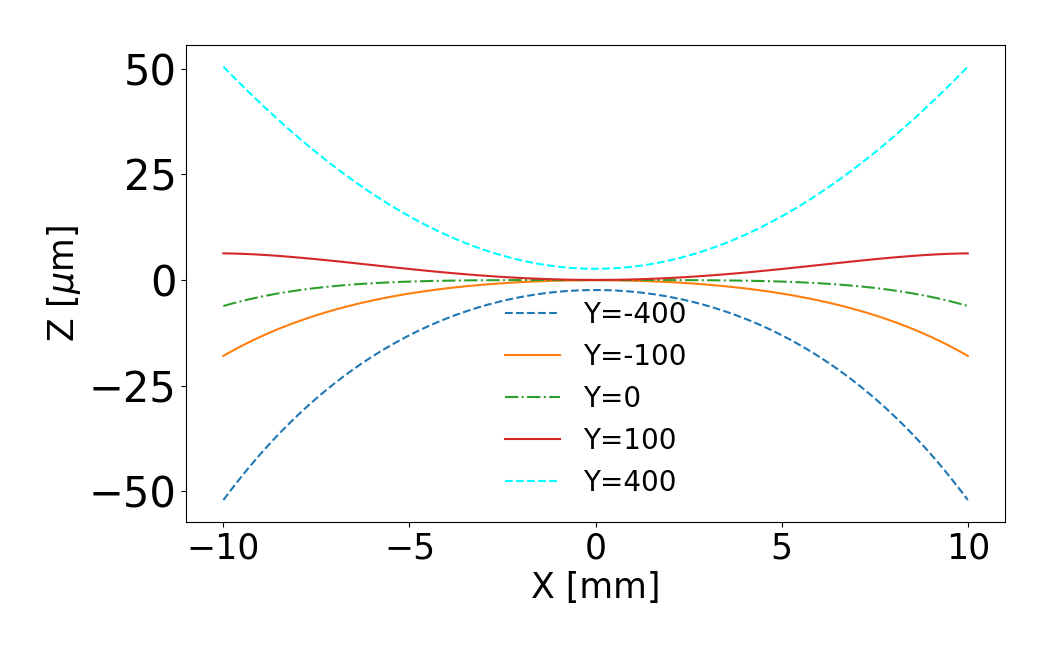
\includegraphics[width=0.32\textwidth]{figures/diaboloid_detrended_5mrad_1:5_profile.png}
% 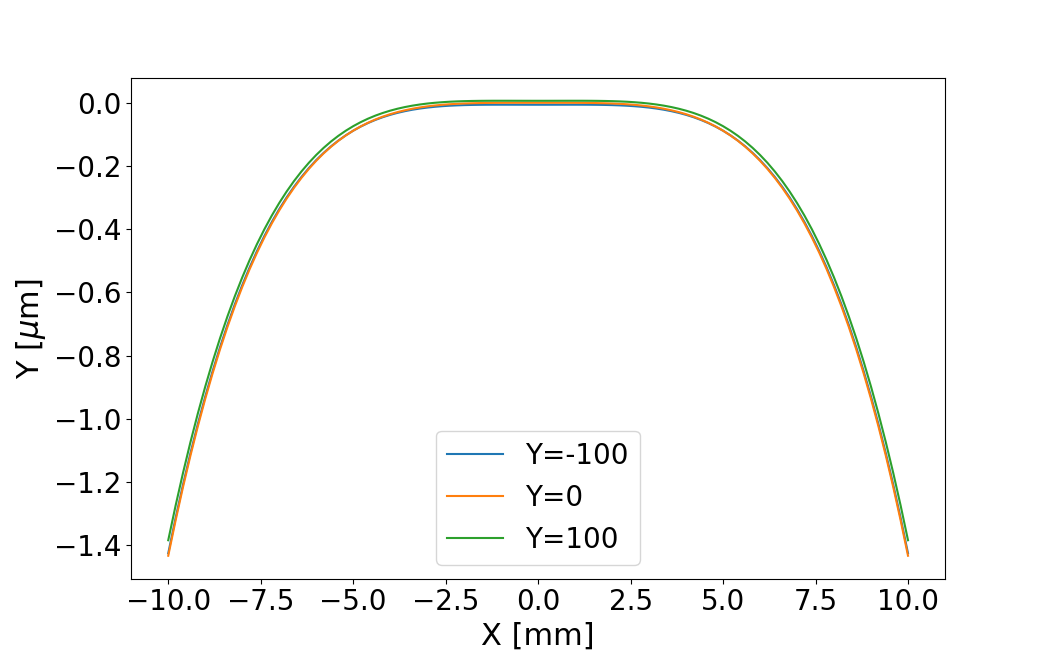
\includegraphics[width=0.32\textwidth]{figures/diaboloid_detrended_5mrad_1:2_profile.png}
% 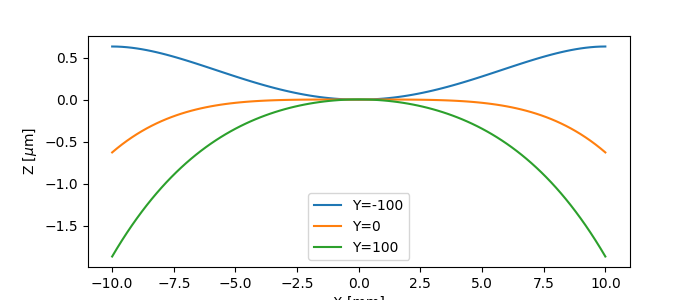
\includegraphics[width=0.32\textwidth]{figures/diaboloid_detrended_5mrad_1:1_profile.png}
% 
% \caption{
% Same as Fig.~\ref{fig:detrended} but for an incident angle of 5 mrad (instead of 2 mrad). The detrended toroid major radii are R$_{a)}$=1.6 Km, R$_{b)}$=4 Km, R$_{c)}$=8 Km and minor radii r$_{a)}$=33.3 mm, r$_{b)}$=66.6 mm, r$_{c)}$=100 mm.
% }
% \end{figure}



We apply this analysis to the case of the beamline 12.2.2 studied before. For the upgraded ALS-U storage ring, the beamline produced a spot size of 14 $\times$ 42 $\mu$m$^2$ (H $\times$ V) with a toroidal mirror in M2 (Fig.~\ref{fig:als}a$_2$), and this would become 10 $\times$ 18 $\mu$m$^2$ with a diaboloid (Fig.~\ref{fig:als}b$_2$). As the situation is close to the 2:1 demagnification and the incidence angle is 2 mrad, this is an interesting case for upgrading the mirror to an approximated diaboloid. Fig.~\ref{fig:detrendedBeamline}a show the diaboloid profile with a toroid detrended. 


\begin{figure}\label{fig:detrendedBeamline}
\flushleft
a)~~~~~~~~~~~~~~~~~~~~~~~~~~~~~~~~~b)~~~~~~~~~~~~~~~~~~~~~~~~~~~~~~c)\\
\centering
\includegraphics[width=0.32\textwidth]{figures/diaboloid_bl1222_detrended_image.png} 
\includegraphics[width=0.32\textwidth]{figures/linearizedparaboliccone_bl1222_detrended_image.png} 
\includegraphics[width=0.32\textwidth]{figures/ellipticalcylinder_bl1222_detrended_image.png} 

\includegraphics[width=0.32\textwidth]{figures/diaboloid_bl1222_detrended_profile.png}
\includegraphics[width=0.32\textwidth]{figures/linearizedparaboliccone_bl1222_detrended_profile.png}
\includegraphics[width=0.32\textwidth]{figures/ellipticalcylinder_bl1222_detrended_profile.png}

\caption{Surface shapes for BL 12.2.2 with a toroid detrended and selected sagittal profiles.
a) Diaboloid, b) cone (Eq.~\ref{eq:sagRadius}). c) Elliptical cylinder bent to a parabola. The detrended toroid major radius is R=8.075 Km and the minor radius is  r=22.595 mm.
}
\end{figure}

Two approximated solutions are studied by ray tracing. First, using a substrate with a circular sagittal section with radius that linearly changes along the $Y$ (tangential) direction Fig.~\ref{fig:detrendedBeamline}b as indicated in Eq.~\ref{eq:sagRadius} (cone). The second one, more precise at a first view, would consist in pre-shaping a cylinder with elliptical (sagittal) section that is the exact sagittal profile at $Y$=0 (Fig.~\ref{fig:detrendedBeamline}c).  This cylinder with elliptical section could be envisaged to be manufactured with sufficient accuracy. 

The spot size produced by the diaboloid is 10 $\times$ 18 $\mu$m$^2$ (Fig.~\ref{fig:als}b$_2$), and 12 $\times$ 23 $\mu$m$^2$ with the first approximation (cone bent to parabola) (Fig.~\ref{fig:finalcomparison}a). In the case that this cone is degenerated into a cylinder, the size becomes 14 $\times$ 33 $\mu$m$^2$ and an aberration tail appears in vertical (Fig.~\ref{fig:finalcomparison}b). This is due that this beamline is close but not exactly at 1:2 magnification (it is exactly M=$q$:$p$=8.075:18.800). If using the second approximation (cylinder with elliptical section) we obtain: 16 $\times$ 38 $\mu$m$^2$ with aberration tail, for the same reason (Fig.~\ref{fig:finalcomparison}c). Looking at the horizontal direction we see a small background using the shape with circular sagittal section (Fig.~\ref{fig:finalcomparison}a and b) as compared with the cleaner distribution for the elliptical sagittal section (Fig.~\ref{fig:finalcomparison}c). 

We check now the beamline in a perfect 1:2 configuration, by setting $q$=9.4 m. In this configuration the diaboloid gives 12 $\times$ 22 $\mu$m$^2$ (not shown), 13 $\times$ 26 $\mu$m$^2$ for the cone and for the circular cylinder (Fig.~\ref{fig:finalcomparison}d), as expected because for 1:2 magnification the cone degenerates in a cylinder. The result for the elliptical cylinder is similar (not shown), demonstrating that there is no much benefit in this case to shape the cylinder with a more complicated elliptical section.   


In conclusion, all approximations for the diaboloid shape (including the simplest circular cylinder bent to a parabola) work well at exact 2:1 demagnification. However at even small deviations from the 2:1 condition like in the present bl 12.2.2 case, the approximation of the diaboloid by a cone has to be used to eliminate the asymmetric aberration tail in tangential direction. For other magnifications the exact diaboloid should be used.

%approximated sagittal cylinders work well only in 1:2 magnification, and there is no additional benefit to make an elliptical shape with respect to the circular one. .   




\begin{figure}\label{fig:finalcomparison}
\flushleft
a)~~~~~~~~~~~~~~~~~~~~~~~~~~~~~~~~~~~~~~~~~~~~~~~~~b)\\
\centering
\includegraphics[width=0.49\textwidth]{figures/prefinal_approx1.png} 
\includegraphics[width=0.49\textwidth]{figures/prefinal_approx1_linearized.png}\\

\flushleft
c)~~~~~~~~~~~~~~~~~~~~~~~~~~~~~~~~~~~~~~~~~~~~~~~~~d)\\
\centering
\includegraphics[width=0.49\textwidth]{figures/prefinal_approx2.png} 
\includegraphics[width=0.49\textwidth]{figures/prefinal_approx1_exact1over2.png} 
% \flushleft
% a$_2$)~~~~~~~~~~~~~~~~~~~~~~~~~~~~~~~~~b$_2$)~~~~~~~~~~~~~~~~~~~~~~~~~~~~~~c$_2$)\\
% \centering
% \includegraphics[width=0.32\textwidth]{figures/final_approx1.png} 
% \includegraphics[width=0.32\textwidth]{figures/final_approx1_linearized.png} 
% \includegraphics[width=0.32\textwidth]{figures/final_approx2.png}


\caption{ Image produced by bl 12.2.2 with: 
a) Diaboloid approximated by a cone (circular section) bent to a parabola b) Diaboloid approximated by a cylinder (circular section) bent to a parabola c) Diaboloid approximated by a cylinder (elliptical section) bent to a parabola, and d) like b) but in exact 2:1 configuration (M=$q$:$p$=9.4:18.800).
}
\end{figure}


% which would require to pre-shape a cylinder with elliptical cross section instead of the current circular shape. The maximum deviation from the circle is about 25 $\mu$m. For the other cases a linearization of the change would be a good simplification, as the sagittal profiles have similar aspect. The situation changes considerably when going to less grazing angle. Less grazing imply less aberrations and therefore the amplitudes of the height differences between the diaboloid and the toroid are only a few microns (Fig.~\ref{fig:detrended5mrad}). However, the shapes of the profiles change when going from $Y$=-100 mm to $Y$=100 mm, meaning that the linearization does not work \inred{TO BE CHECKED...}. 




% Dear  Friends of the Diaboloid,
% Manolo pointed out numerous discrepancies in my last version of the diaboloid note...........mainly that I had confused type 1 and type 2, ie. point to line and line to point.  We need the latter, type 2.  So I went through all again, and expanded a bit.  The deviation of the diaboloid at the magic 2:1 (as Manolo pointed out, the 2:1 is an approximation.....turns out to be a pretty good one) turns out to be only 1.5 microns at the edge of our aperture.  I get this by just subtracting the surface heights, and then also by an expansion method which directly leads to the x^4 height residual.  So the fact that the shape to be made is a plane ellipse, and it doesn't deviate much from a cylinder makes me hope that this shape can be made.  The off 2:1 case, like the 5:1 demag case where the shape is highly conical is much more problematic.  1.5 microns is doable by the way by differential deposition of Si............its the way that APS used to make plane ellipses, starting with a sphere.  I think the APS and NSLS2 have long computer controlled sputtering machines for making these varying thickness coatings.  You cannot do this in metal as the coatings become very rough.  So in principle this could be done by starting with the cylinder and just putting a variable thickness coating down.............this is done for many other apps.   But, we need good interferometric metrology.  



\section{Summary}
\label{sec:summary}

The diaboloid is a new optical surface that focuses light from infinity to a point in one direction and in the orthogonal direction focuses from the real source to a stigmatic point.  Typically toroidal mirrors serve this purpose, but with the advent of diffraction limited storage rings with very bright bending magnet sources, there is a need for better focusing. The diaboloid provides aberration free focusing and will be useful in all cases where there is a vertically collimating pre-mirror, such as is typical in double-crystal monochromator beamlines. The shape is complex, but in the case of 2:1 horizontal demagnification, devolves to parabolic curvature in the tangential direction and elliptical curvature in the sagittal direction. For 5 mrad grazing angles for typical beamline parameters the deviation of the surface from toroidal is 1-2 microns, and this could open the way to manufacture of the surface by sputtered additional of a thin varied thickness coating.  Additionally, at the 2:1 condition, the unbent surface (the parabolic curvature is added by bending) is essentially a long plane ellipse or a circle, opening up possibilities for normal incidence optical interferometry.  Finally, unlike the toroid, the diaboloid can produce an aberration free image under any magnification, and so offers the possibility of eliminating further downstream demagnification elements. 

%We summarized the basic equations of the diaboloid and its approximations and implemented them in Oasys to perform several ray tracing simulations. 
%The "parabolic-quasicone" (Eq.~\ref{eqn:parabolicCone}), an  approximation to the diaboloid, is also implemented. It may play in the future an important role in applying the diaboloid concept to new beamlines, because it is probably easier to manufacture and polish to enough quality. We studied these mirrors surfaces applied to the ALS beamline 12.2.2 in its present (ALS) and in the Upgraded configuration (ALS-U). It is manifested the possible interest to migrate to diaboloid or parabolic-cone solutions for the ALS-U, if they can be built. The use of these new solutions may also improve the beamline performances because they can be used with high demagnification. We showed that magnifications of 1:5 and up to 1:10 may be used with parabolic-cone or diaboloid mirrors for this beamline. 

% We have derived an exact solution of the diaboloid mirror in the form
% \begin{equation}
% \label{eqn:summary_form}
% z(x,y) = - \sqrt{A - B y - C \sqrt{x^2 + (y - D)^2}},
% \end{equation}
% in the coordinate system where the source beam is inclined downward at an angle of $2 \theta$, and $x$ and $y$ are rooted at the mirror center. The complete expression for $z(x,y;p,q,\theta)$ is given in Eq. \ref{eqn:7new_z}. It remains to test this exact expression against existing series representations (from McKinney), and through ray-trace beamline modeling.



     %-------------------------------------------------------------------------
     % The back matter of the paper - acknowledgements and references
     %-------------------------------------------------------------------------

     % Acknowledgements come after the appendices

\section{Acknowledgements}       
 
 
This work was supported by the Director, Office of Science, Office of Basic Energy Sciences, of the U.S. Department of Energy under Contract No. DE-AC02-05CH11231.



     % References are at the end of the document, between \begin{references}
     % and \end{references} tags. Each reference is in a \reference entry.

% \begin{references}
% \reference{Author, A. \& Author, B. (1984). \emph{Journal} \textbf{Vol}, 
% first page--last page.}
% \end{references}
%\cite{knuth84}

%% Note added by Overleaf: If using bibtex, remove the "references" environment above, and uncomment the following line.
\referencelist{iucr}


%      %-------------------------------------------------------------------------
%      % TABLES AND FIGURES SHOULD BE INSERTED AFTER THE MAIN BODY OF THE TEXT
%      %-------------------------------------------------------------------------
% 
%      % Simple tables should use the tabular environment according to this
%      % model
% 
% \begin{table}
% \caption{Caption to table}
% \begin{tabular}{llcr}      % Alignment for each cell: l=left, c=center, r=right
%  HEADING    & FOR        & EACH       & COLUMN     \\
% \hline
%  entry      & entry      & entry      & entry      \\
%  entry      & entry      & entry      & entry      \\
%  entry      & entry      & entry      & entry      \\
% \end{tabular}
% \end{table}
% 
%      % Postscript figures can be included with multiple figure blocks
% 
% \begin{figure}
% \caption{Caption describing figure.}
% \includegraphics{fig1}
% \end{figure}


\end{document}                    % DO NOT DELETE THIS LINE
%%%%%%%%%%%%%%%%%%%%%%%%%%%%%%%%%%%%%%%%%%%%%%%%%%%%%%%%%%%%%%%%%%%%%%%%%%%%%%


